% This is samplepaper.tex, a sample chapter demonstrating the
% LLNCS macro package for Springer Computer Science proceedings;
% Version 2.20 of 2017/10/04
%
\documentclass[runningheads]{llncs}
%
\usepackage{graphicx}
\usepackage{algorithm}
%\usepackage{algorithmic}
\usepackage{algpseudocode}
\usepackage{amssymb}
\usepackage{amstext}
\usepackage{graphicx}
%\usepackage{subfigure}
%\usepackage{subcaption}
\usepackage{color}
\usepackage{todonotes}
%\usepackage{times}
%\captionsetup{compatibility=false}



\newcommand{\ecall}{\mathsf{C}}
\newcommand{\eresp}{\mathsf{R}}
\newcommand{\ewrite}{\mathsf{Wr}}
\newcommand{\eread}{\mathsf{Rd}}
\newcommand{\ecas}{\mathsf{CAS}}
\newcommand{\trace}{\mathit{Tr}}
\newcommand{\pair}[1]{{\langle{#1}\rangle}}
\newcommand{\set}[1]{\left\{{#1}\right\}}

\newcommand{\p}{\mathbb{P} }
\newcommand{\ft}{S_f}
\newcommand{\ct}{S_c}
\newcommand{\se}{\mathit{I_e}}
\newcommand{\var}{\mathit{Var}}
\newcommand{\ce}{\mathit{M_e}}
\newcommand{\dr}{\mathsf{D}}

\newtheorem{myTheo}{Theorem}
\newtheorem{myDef}{Definition}

%\newenvironment{example}[1][Example]{\begin{trivlist}
%\item[\hskip \labelsep {\bfseries #1}]}{\end{trivlist}}

\newcommand{\wri}{\mathtt{write}}
\newcommand{\rea}{\mathtt{read}}
\newcommand{\hb}{\textit{happen-before }}

\usepackage{wrapfig}
\usepackage{subfigure}
% Used for displaying a sample figure. If possible, figure files should
% be included in EPS format.
%
% If you use the hyperref package, please uncomment the following line
% to display URLs in blue roman font according to Springer's eBook style:
% \renewcommand\UrlFont{\color{blue}\rmfamily}

\begin{document}
%
\title{Interleaving-tree Based Fine-grained Linearizability Fault Localization}
%
\titlerunning{Interleaving-tree Based Fine-grained Linearizability Fault Localization}
% If the paper title is too long for the running head, you can set
% an abbreviated paper title here
%
\author{Yang Chen\inst{1,2} \and
Zhenya Zhang\inst{3}\thanks{The work was partially done when the author was a student at Institute of Software, Chinese Academy of Sciences} \and
Peng Wu\inst{1,2}\and
Yu Zhang\inst{1,2}}
%
\authorrunning{Y. Chen et al.}
% First names are abbreviated in the running head.
% If there are more than two authors, 'et al.' is used.
%
\institute{{State Key Laboratory of Computer Science\\Institute of Software, Chinese Academy of Sciences}\and
University of Chinese Academy of Sciences\and
National Institute of Informatics
}
%
\maketitle              % typeset the header of the contribution
%
\begin{abstract}
Linearizability is an important correctness criterion for concurrent objects. Existing work mainly focuses on linearizability verification of coarse-grained traces with operation invocations and responses only. However, when linearizability is violated, such coarse-grained traces do not provide sufficient information for reasoning about the underlying concurrent program faults. In this paper, we propose a notion of \textit{critical data race sequence} (\textit{CDRS}), based on our fine-grained trace model, to characterize concurrent program faults that cause violation of linearizability. We then develop a labeled tree model of interleaved program executions and show how to identify \textit{CDRS}es and localize concurrent program faults automatically with a specific node-labeling mechanism. We also implemented a prototype tool, FGVT, for real-world Java concurrent programs. Experiments show that our localization technique is effective, i.e., all the \textit{CDRS}es reported by FGVT indeed reveal the root causes of linearizability faults.

\keywords{Linearizability  \and Bug localization \and Concurrency \and Testing}
\end{abstract}
%
%
%
%\section{Introduction}\label{sec:introduction}
Localization of concurrency faults has been a hot-spotted topic for long time.
Multiple trials for the same concurrent programs with the same inputs usually result in different outputs.
This nature of concurrent program executions is known as nondeterminism. Due to it, 
it is non-trivial to decide whether a concurrent program is potential to go wrong.
Moreover, even if a concurrent program has been known buggy, 
it is difficult to reproduce the same fault or address the root cause of the fault.

There have been many techniques addressing the problem of localization of concurrency fault. The very basic way is to
exhaust the \textit{thread scheduling} space to replay and analyze the buggy execution.
%and these works mainly aim to replay and locate concurrency faults through recording and intervening \textit{thread scheduling}. 
Thread scheduling is usually described as a sequence of thread identifiers that reflects the order of thread executions and context switches.
 In \cite{Choi2000Deterministic,DBLP:journals/concurrency/EdelsteinFGNRU03,DBLP:journals/entcs/Stoller02}, 
 the thread schedule in one buggy execution is recorded and then used to reproduce the same bugs during the rerun. 
 In many literatures, there is also another notion called \textit{fine-grained trace} that is usually defined as a sequence of memory access instructions and 
 also corresponds to one specific thread schedule.
 In \cite{DBLP:conf/issta/KhoshnoodKW15}, 
 fine-grained traces and correctness criteria are encoded as logical formulas to diagnose and repair concurrency bugs through model checking. 
 Generally, such fine-grained investigation suffers from a serious problem of state space explosion, and
 there are many works specifically addressing this issue to accelerate the localization process, such as the heuristic rules based work
 \cite{Ben2003Heuristics}, iterative context bounding \cite{DBLP:conf/pldi/MusuvathiQ07}. 
 However, the targets of most of the aforementioned works are general concurrency faults, without consideration towards the nature of some specific concurrency fault.

In this paper, we consider the linearizability correctness criterion. Linearizability \cite{DBLP:journals/toplas/HerlihyW90} is a widely-accepted correctness criterion for concurrent data structures or concurrent objects. 
Intuitively, it means that every operation on a shared object appears to take effect instantaneously at some point, called \textit{linearization point}, 
between the invocation and response of the operation, and the behavior exposed by the sequence of operations serialized at their linearization points must conform to the sequential specification of the shared object.


Linearizability verification is a hot-spotted topic in the recent years' research of concurrency. There are large numbers of works and tools such as
\cite{DBLP:conf/popl/BouajjaniEEH15,DBLP:conf/pldi/BurckhardtDMT10,DBLP:conf/popl/BouajjaniEEH15,DBLP:conf/forte/HornK15a,DBLP:conf/sac/LongZ16,DBLP:journals/concurrency/Lowe17}, 
focusing on the linearizability verification of the given traces based on a coarse-grained trace model.
Usually the traces in such works are described as a partial order set of object methods, and the basic approach 
for linearizability checking is to enumerate the possible topologically sorted sequential traces that satisfy the correctness criteria of the specific data structures.
This approach also suffers from the state space explosion problem in the other level compared to the fine-grained localization work, and thus
most of the existing works propose acceleration strategies to address this problem.
Furthermore, since the coarse-grained model only investigates composed of method invocations and responses, 
no information about root causes of linearizability faults is provided by these techniques. 
Generally, these techniques emphasize acceleration towards the state space explosion problem rather than analysis or localization of linearizability faults.
%but still suffers from the state space explosion problem. Moreover, even when a violation of linearizability is detected, no clue to its root cause is provided by these techniques. A coarse-grained trace is composed only of operation invocations and responses, hence keeps the fine-grained memory access events away from being investigated in reasoning about linearizability faults.



 This paper mainly addresses the issue of the relation between data race and linearizability faults. 
 We propose a notion called \textit{Critical Data Race Sequence} (\textit{CDRS}) based on a fine-grained trace model. 
 Intuitively, a CDRS contains a sequence of data races that decisively result in linearizability faults, 
 and thus the existence of CDRSes implies that the concurrent program is potential to produce non-linearizable traces. 
 Furthermore, in order to identify CDRSes, we model all the possible fine-grained traces of a concurrent execution as an \textit{interleaving tree}, 
 where each node corresponds to a data race and each path from the root to a leaf node corresponds to a fine-grained trace. 
 We label each node with a pre-defined symbol depending on the linearizability of all the paths passing through the node, and 
 then the existence of CDRSes can be determined by the certain pattern of node sequences in the labeled interleaving tree.


In order to resolve the state space explosion problem, we divide the localization process into a coarse-grained level and a fine-grained level.
The coarse-grained level addresses the issue of working out a test case that contains a small number of operations but is sufficient to trigger a linearizability faults \cite{DBLP:conf/seke/ZhangWZ17}. 
Then, given the small test case as the input
for the fine-grained level localization, the number of memory access instructions that should be investigated 
can be hugely reduced.
Together with a linearizability checking technique \cite{DBLP:journals/concurrency/Lowe17} and coarse-grained localization \cite{DBLP:conf/seke/ZhangWZ17}, the overall process is illustrated as in Fig.\ref{fig:liucheng}, in which C is the main contribution of this work.

\vspace{-0.5cm}
\begin{figure}[!ht]
\centering
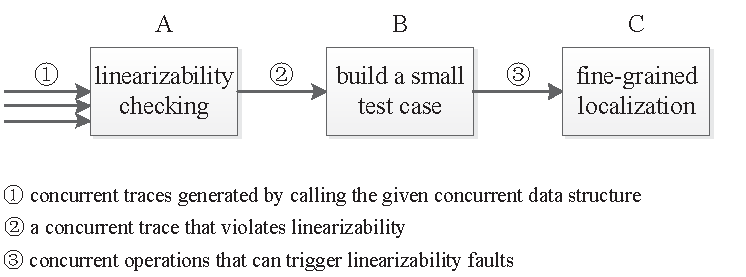
\includegraphics[width = 3.5in]{liucheng.eps}
\caption{Labels of nodes}\label{fig:liucheng}
\end{figure}
\vspace{-0.5cm}

\noindent\textbf{\textit{Contributions.}}
The contributions of this paper are as follows:
\begin{itemize}
  \item We extend the traditional coarse-grained trace model to a fine-grained trace model by adding memory access events. We also extend the notion of linearizability onto fine-grained traces.
  \item We propose the key notion of \textit{Critical Data Race Sequence} (CDRS) for characterizing the data races that are decisive to linearizability faults.
  \item We develop a labeled interleaving tree model that contains all the possible fine-grained traces of a concurrent execution. Each node corresponds to a data race and is labeled in a way that can reflect the existence of CDRS through a certain pattern.
  \item We implement a prototype tool, \textit{FGVT}, for real-world Java concurrent programs. Experiments show that FGVT is effective, in that all the CDRSes reported by FGVT indeed reveal the root causes of linearizability faults.
\end{itemize}

\noindent\textbf{\textit{Related work.}} Automated linearizability checking algorithms were presented in \cite{DBLP:conf/pldi/BurckhardtDMT10,DBLP:journals/jpdc/WingG93}, but suffered from a bottleneck of performance. Based on \cite{DBLP:journals/jpdc/WingG93}, optimized algorithms were proposed in \cite{DBLP:journals/concurrency/Lowe17} and \cite{DBLP:conf/forte/HornK15a} through partial order reduction and compositional reasoning, respectively. Model checking was applied in \cite{DBLP:conf/popl/BouajjaniEEH15,DBLP:conf/pldi/EmmiEH15} for linearizability checking, with simplified first-order formulas that can help improve efficiency. Fine-grained traces were introduced in \cite{DBLP:conf/sac/LongZ16} to accelerate linearizability checking. All these work lays a firm foundation for the localization of linearizability faults.

Efforts have been devoted on concurrency bug localization, e.g., through an active-testing approach based on bug patterns. The potential bug locations can then be ranked with the suspicious bug patterns gathered. The characteristics of bug patterns were discussed in \cite{DBLP:conf/asplos/LuPSZ08,DBLP:conf/ipps/FarchiNU03} in details. Memory access patterns were proposed in \cite{DBLP:conf/icse/ParkVH10,DBLP:conf/icst/ParkVH12,DBLP:conf/icsm/LiuQWM14} for ranking bug locations. A fault comprehension technique was further presented in \cite{DBLP:conf/icse/Park04} for bug patterns. Definition-use invariants were presented in \cite{DBLP:conf/oopsla/ShiPYLZCZ10} for detecting concurrency bugs with pruning and ranking methods. A constraint-based symbolic analysis method was proposed in \cite{DBLP:conf/issta/KhoshnoodKW15} to diagnose concurrency bugs.

Some other concurrency bug localizations techniques were based on the bug localization techniques for sequential programs. In \cite{DBLP:conf/IEEEpact/GottschlichPPW13}, concurrent predicates were derived from an assertion mechanism to determine whether a data race causes a concurrency bug. Concurrent breakpoints, an adaption of a breakpoint mechanism, were proposed in \cite{DBLP:conf/ppopp/ParkS12} for concurrent program debugging.

We claim that the novelty of this work is that we focus on the correctness criterion of linearizability, and thus tree search also focuses on such a direction. We apply some 
existing tree search techniques such as partial-order reduction but we emphasizes our novel approach of localizing linearizability faults.


\noindent\textbf{\textit{Organization.}} The rest of the paper is organized as follows. Section \ref{sec:motivatingeg} presents an example to illustrate our motivation. Section \ref{sec:fgtracemodel} introduces our fine-grained trace model. Section \ref{sec:criticaldataraces} presents the key notion of CDRS based on our fine-grained trace model. Section \ref{sec:intertree} shows the labeled interleaving tree model, and the pattern of CDRSes. Section \ref{sec:implementation} reports the implementation and experiments about our prototype tool FGVT. Section \ref{sec:conclusion} concludes the paper.

\section{Motivating Example}\label{sec:motivatingeg}

In this section, we illustrate the motivation of this work through a buggy concurrent data structure \textit{PairSnapShot} \cite{DBLP:conf/sac/LongZ16}.

\begin{wrapfigure}[15]{r}{0.55\textwidth}
\centering
    \begin{small}
 \vspace{-0.8cm}
        \begin{verbatim}
    PairSnapShot:
        int d[2];
        write(i,v){
            d[i] = v;                #1
        }
        Pair read(){
            while(true){
                int x = d[0];        #2
                int y = d[1];        #3
                if(x == d[0])        #4
                    return <x,y>;
            }
        }
        \end{verbatim}
        \vspace{-1cm}
        \end{small}
        \caption{A concurrent data structure: PairSnapShot}
        \label{fig:pairsnapshot}
\end{wrapfigure}


Fig.\ref{fig:pairsnapshot} shows a simplified version of PairSnapShot, where it holds an array \texttt{d} of size 2. A \texttt{write(i,v)} operation writes \texttt{v} to \texttt{d[i]}, while a \texttt{read} \texttt{$\to \langle v_0,v_1\rangle$} operation reads the values of \texttt{d[0]} and \texttt{d[1]}, which are $v_0$ and $v_1$, respectively.

 A correctness criterion of PairSnapShot is that \texttt{read} should always return the values of the same moment. However, 
Fig. \ref{fig:psscoarsetrace} shows a concurrent execution in which the return values of \texttt{read} do not exist at any moment of the execution. 
In Fig.~\ref{fig:psscoarsetrace}, time moves from left to right; dark lines indicate the time intervals of operations and  
the short vertical lines at the both ends of a dark line represent the moment when an operation is invoked and returned, respectively.
A label ${t:(v_0,v_1)}$ indicates that at the moment $t$,  \texttt{d[0]} is $v_0$ and \texttt{d[1]} is $v_1$.
  The operation \texttt{read()} on Thread 2 returns a value $\mathtt{\pair{1,2}}$,
  which is not consistent with value of any moment. 
  %The `\texttt{x}' labels in Fig.\ref{fig:pairsnapshot} mark the moments when each instruction takes effects, which explains exactly the cause of the linearizability fault.

The reason of this violation can be found out by enumerating the possible executing orders of memory access events which is labeled by \texttt{\#} in Fig.~{}. 
One possible order that can trigger the violation is illustrated in Fig.~{}, in which ``\texttt{x}'' indicate the executing moments of the corresponding memory access events. 
Actually, this model checking approach is the most common way to locate the root cause of concurrency bugs, and has been studied in many existing literatures.
Here, our focus is not on how to find this fine-grained executing order, but to study how the thread execution order, in which data race exists, influences the final result of linearizability.

%The fine-grained root cause can be explained by the temporal order of instructions labeled by ``\texttt{x}''. Since \texttt{d[0]} and \texttt{d[1]} should be considered as a whole (a pair), instructions in \texttt{write} and \texttt{read} should accordingly be considered accessing the whole pair, and thus data races exist there. In this execution, all data races between instructions of \texttt{write} and \texttt{read} together result in the linearizability fault, and all ones are necessary to trigger the linearizability fault.



\begin{figure}[!ht]
\centering
\setlength{\unitlength}{0.8cm}
\begin{picture}(10,2.5)
\thinlines

\multiput(1.7,1.5)(0.2,0){44}{\line(1,0){0.1}}
\thicklines
\put(2.0,1.5){\line(1,0){1.7}}
\put(4.1,1.5){\line(1,0){1.7}}
\put(6.2,1.5){\line(1,0){1.7}}
\put(8.3,1.5){\line(1,0){1.7}}
\begin{small}
\put(0,1.4){Thread 1}
\put(1.9,1.7){$\mathtt{write(0,2)}$}
\put(4.0,1.7){$\mathtt{write(1,2)}$}
\put(6.1,1.7){$\mathtt{write(1,1)}$}
\put(8.2,1.7){$\mathtt{write(0,1)}$}
\put(0,0.4){Thread 2}

\put(1.0,2.3){$t_1:\pair{1,1}$}
\put(3.0,2.3){$t_2:\pair{2,1}$}
\put(5.0,2.3){$t_3:\pair{2,2}$}
\put(7.1,2.3){$t_4:\pair{2,1}$}
\put(9.2,2.3){$t_5:\pair{1,1}$}

\thinlines

\multiput(1.7,0.5)(0.2,0){44}{\line(1,0){0.1}}
\thicklines
\put(2.3,0.5){\line(1,0){7.5}}
\put(4.6,0.7){\color{red}{$\mathtt{read\to \pair{1,2}}$}}

\put(2.3,0.4){\line(0,1){0.2}}
\put(9.8,0.4){\line(0,1){0.2}}

\put(2.0,1.4){\line(0,1){0.2}}
\put(4.1,1.4){\line(0,1){0.2}}
\put(6.2,1.4){\line(0,1){0.2}}
\put(8.3,1.4){\line(0,1){0.2}}

\put(3.7,1.4){\line(0,1){0.2}}
\put(5.8,1.4){\line(0,1){0.2}}
\put(7.9,1.4){\line(0,1){0.2}}
\put(10,1.4){\line(0,1){0.2}}

\thinlines
\multiput(1.8,0.3)(0,0.2){10}{\line(0,1){0.1}}
\multiput(3.9,0.3)(0,0.2){10}{\line(0,1){0.1}}
\multiput(6.0,0.3)(0,0.2){10}{\line(0,1){0.1}}
\multiput(8.1,0.3)(0,0.2){10}{\line(0,1){0.1}}
\multiput(10.2,0.3)(0,0.2){10}{\line(0,1){0.1}}





\end{small}
\end{picture}
\caption{A buggy trace of PairSnapShot}
\label{fig:psscoarsetrace}
\end{figure}


\vspace{-1cm}

\begin{figure}[!ht]
\centering
\setlength{\unitlength}{0.8cm}
\begin{picture}(10,2.5)
\thinlines

\multiput(1.7,1.5)(0.2,0){44}{\line(1,0){0.1}}

\begin{small}
\put(0,1.4){Thread 1}

\put(0,0.4){Thread 2}

\put(1.0,2.3){$t_1:\pair{1,1}$}
\put(3.0,2.3){$t_2:\pair{2,1}$}
\put(5.0,2.3){$t_3:\pair{2,2}$}
\put(7.1,2.3){$t_4:\pair{2,1}$}
\put(9.2,2.3){$t_5:\pair{1,1}$}

\thinlines

\multiput(1.7,0.5)(0.2,0){44}{\line(1,0){0.1}}





\thinlines
\multiput(1.8,0.3)(0,0.2){10}{\line(0,1){0.1}}
\multiput(3.9,0.3)(0,0.2){10}{\line(0,1){0.1}}
\multiput(6.0,0.3)(0,0.2){10}{\line(0,1){0.1}}
\multiput(8.1,0.3)(0,0.2){10}{\line(0,1){0.1}}
\multiput(10.2,0.3)(0,0.2){10}{\line(0,1){0.1}}




\put(3.0,1.4){\texttt{x}}
\put(4.6,1.4){\texttt{x}}
\put(6.6,1.4){\texttt{x}}
\put(8.8,1.4){\texttt{x}}

\put(2.7,0.4){\texttt{x}}
\put(5.4,0.4){\texttt{x}}
\put(9.3,0.4){\texttt{x}}



\put(2.3,0.4){\line(0,1){0.2}}
\put(9.8,0.4){\line(0,1){0.2}}

\put(2.0,1.4){\line(0,1){0.2}}
\put(4.1,1.4){\line(0,1){0.2}}
\put(6.2,1.4){\line(0,1){0.2}}
\put(8.3,1.4){\line(0,1){0.2}}

\put(3.7,1.4){\line(0,1){0.2}}
\put(5.8,1.4){\line(0,1){0.2}}
\put(7.9,1.4){\line(0,1){0.2}}
\put(10,1.4){\line(0,1){0.2}}

\put(2.1,0.1){$c_r$}
\put(9.8,0.1){$r_r$}

\end{small}
\begin{scriptsize}

\put(2.9,1.1){\texttt{\#1}}
\put(4.6,1.1){\texttt{\#1}}
\put(6.6,1.1){\texttt{\#1}}
\put(8.8,1.1){\texttt{\#1}}

\put(2.7,0.1){\texttt{\#2}}
\put(5.4,0.1){\texttt{\#3}}
\put(9.3,0.1){\texttt{\#4}}

\put(2.0,1.1){$c_{w1}$}
\put(4.0,1.1){$c_{w2}$}
\put(6.0,1.1){$c_{w3}$}
\put(8.1,1.1){$c_{w4}$}

\put(3.4,1.1){$r_{w1}$}
\put(5.4,1.1){$r_{w2}$}
\put(7.5,1.1){$r_{w3}$}
\put(9.6,1.1){$r_{w4}$}
\end{scriptsize}

\end{picture}
\caption{An executing order of memory access events triggering the violation in Fig.~{\ref{fig:psscoarsetrace}}}
\label{fig:pssfinetrace}
\end{figure}




\vspace{-0.5cm}

\section{Preliminary}\label{sec:fgtracemodel}


In this section, we extend the traditional coarse-grained trace model \cite{DBLP:conf/popl/BouajjaniEEH15}, recalled in Section \ref{sec:coarsegraintm}, to the fine-grained trace model presented in Section \ref{sec:finegraintm}. Compared to the traditional one, our new model includes memory access instructions such as \texttt{read, write} and atomic primitive \textit{compare-and-swap} (\texttt{CAS}). This enables us to reason about the causes of linearizability faults on the fine-grained level.

\subsection{Coarse-grained trace model}\label{sec:coarsegraintm}
A \textit{trace} $S$ is a finite sequence of events, and each event is in the form $e(\mathit{Arg})^{\left\langle o,t\right\rangle}$, where $e$ is an event symbol ranging over a pre-defined set $E$, $\mathit{Arg}$ represents arguments, $o$ belongs to a set $O$ of operation identifiers and $t$ belongs to a set $T$ of thread identifiers. In our coarse-grained trace model, the set $E$ contains the following subsets:
\begin{itemize}
  \item $\ecall$ contains symbols that represent operation invocation events. An invocation event is represented as $c(v_a)^{\langle o,t\rangle}$ $(c\in \ecall)$, where $v_a$ is the argument of the operation;
  \item $\eresp$ contains symbols that represent operation response events. A response event is represented as $r(v_r)^{\langle o,t\rangle}$ $(r\in \eresp)$, where $v_r$ is the return value of the operation.
\end{itemize}
\noindent We also use $\ecall, \eresp$ to represent the set of corresponding events indiscriminately, and symbol $e\in \ecall\cup \eresp$ to represent an event. The order relation between events in a trace $S$ is written as $\prec_S$ (or $\prec$), i.e., $e_1\prec_S e_2$ if $e_1$ is ordered before $e_2$ in $S$. We denote the operation identifier of an event $e$ as $\mathtt{op}(e)$, and thread identifier as $\mathtt{td}(e)$. An invocation event $c\in \ecall$ and a response event $r\in \eresp$ \textit{match} if $\mathtt{op}(c) = \mathtt{op}(r)$, written as $c\diamond r$. A pair of matching events forms an operation with an operation identifier in $O$, and we represent an operation as $m(v_a)\to v_r$, where $m$ is the operation name.
 A trace $S = e_1e_2\cdots e_n$ is \textit{well-formed} if it satisfies that:
\begin{itemize}
  \item Each response is preceded by a matching invocation:\\
  $e_j\in \eresp$ implies $e_i \diamond e_j$ for some $i<j$
  \item Each operation identifier is used in at most one invocation/response:\\
  $\mathtt{op}(e_i)=\mathtt{op}(e_j)$ and $i<j$ implies $e_i \diamond e_j$
\end{itemize}
 A well-formed trace $S$ can also be treated as a partial order set $\pair{S,\sqsubset_S}$ of operations on \textit{happen-before} relation $\sqsubset_S$ between operations, where $S$ is called a \textit{coarse-grained trace} (or \textit{coarse-grained history}). The \textit{happen-before} relation $\sqsubset_S$ is defined as that: assuming two operations $O_1,O_2$ in $S$ are formed by $c_1,r_1$ and $c_2,r_2$ respectively, then $O_1\sqsubset_S O_2$ if and only if $r_1\prec c_2$.

\begin{example}
Fig.~\ref{fig:psscoarsetrace} shows such a well-formed trace:
$S = c_{w1}c_rr_{w1}c_{w2}r_{w2}c_{w3}r_{w3}c_{w4}r_{r}r_{w4}$, where $c_{wi}$ and $r_{wi}$
represents the invocation and response events of the $i$-th $\mathtt{write}$ operation respectively, and
$c_r$ and $r_r$ represent the invocation and response events of the $\mathtt{read}$ operation.

It is obvious that \begin{small}$\wri(0,2)\prec \wri(1,2)\prec \wri(1,1)\prec \wri(0,1)$\end{small}, 
but there is no \hb  
relation between the $\rea$ operation and anyone of the $\wri$ operations.

\end{example}




A coarse-grained trace $S$ is \textit{sequential} if $\sqsubset_S$ is a total order. 
We define that a \textit{specification} of an object is the set of all sequential traces that satisfy the correctness criteria of that object. 
Note that here correctness criterion is specified by concurrent data structures, such as \textit{first-in-first-out} for \textit{FIFO-Queue}, \textit{first-in-last-out} for \textit{Stack}.

\vspace{-0.2cm}
\begin{myDef}[Linearizability]\label{def:linearizability}
A coarse-grained trace $S$ of an object is linearizable if there exists a sequential trace $S'$ in the specification of the object such that:
\begin{enumerate}
  \item $S$ and $S'$ are composed of the same operations;
  \item $\sqsubset_S \subseteq \sqsubset_S'$, i.e., if $O_1\sqsubset_S O_2$, then $O_1\sqsubset_{S'} O_2$.
\end{enumerate}
\end{myDef}
\vspace{-0.2cm}

Note that this definition speaks only complete traces, neglecting the existence of pending operations, that is, the operations without response events. Since this paper focuses on analysis of linearizability faults rather than detection, we consider complete traces only.

\vspace{-0.1cm}
\begin{example}
Fig.~\ref{fig:accounttwoseqtraces} shows five sequential traces that satisfy requirements 1) and 2) in Definition \ref{def:linearizability} with respect to the coarse-grained trace shown in Fig~\ref{fig:psscoarsetrace}. However, neither of them satisfies the correctness criteria of \textit{PairSnapShot}, which means that neither of them belongs to the specification set of \textit{PairSnapShot}, so we can say that the coarse-grained trace in Fig.~\ref{fig:psscoarsetrace} is non-linearizable.

\end{example}
\vspace{-0.7cm}

\begin{figure}
\centering
\setlength{\unitlength}{0.5cm}
    \begin{picture}(17.5,5)
    \begin{footnotesize}
	\put(0,4.5){$1: \mathtt{read\to \pair{1,2}}$ $\mathtt{write(0,2)}$ $\mathtt{write(1,2)}$ $\mathtt{write(1,1)}$ $\mathtt{write(0,1)}$}
	
	\put(0,3.5){$2: \mathtt{write(0,2)}$ $\mathtt{read\to \pair{1,2}}$ $\mathtt{write(1,2)}$ $\mathtt{write(1,1)}$ $\mathtt{write(0,1)}$}
	
	\put(0,2.5){$3: \mathtt{write(0,2)}$ $\mathtt{write(1,2)}$ $\mathtt{read\to \pair{1,2}}$  $\mathtt{write(1,1)}$ $\mathtt{write(0,1)}$}
	
	\put(0,1.5){$4: \mathtt{write(0,2)}$ $\mathtt{write(1,2)}$ $\mathtt{write(1,1)}$ $\mathtt{read\to \pair{1,2}}$ $\mathtt{write(0,1)}$}
	
	\put(0,0.5){$5: \mathtt{write(0,2)}$ $\mathtt{write(1,2)}$ $\mathtt{write(1,1)}$ $\mathtt{write(0,1)}$ $\mathtt{read\to \pair{1,2}}$}
	\end{footnotesize}
    \end{picture}
    \vspace{-0.5cm}

    \caption{Five possible sequential traces}\label{fig:accounttwoseqtraces}
\end{figure}
\vspace{-0.5cm}

\subsection{Fine-grained trace model}\label{sec:finegraintm}


In addition to $\ecall$ and $\eresp$, the symbol set $E$ has other subsets of events in our fine-grained trace model:

\begin{itemize}
  \item $\ewrite$ contains symbols that represent the \textit{memory writing} events. An event of memory writing is represented as $wr(addr,v)^{\left\langle o,t\right\rangle}$ $(wr \in \ewrite)$, where $addr$ is the memory location to be modified to a value $v$;
  \item $\eread$ contains symbols that represent the \textit{memory reading} events. An event of memory reading is represented as $rd(addr)^{\left\langle o,t\right\rangle}$ $(rd \in \eread)$, where $addr$ is the memory location to be read;
  \item $\ecas$ contains symbols that represent the \textit{atomic primitive}, such as \textit{compare-and-swap} (\textit{CAS}) in modern architecture. A \textit{CAS} event can be represented as $cas(addr, v_e, v_n)^{\left\langle o,t\right\rangle}$ $(cas \in \ecas)$, where $addr$ represents a memory location, $v_e$ and $v_n$ are two values. The function of this atomic primitive is that if the value at $addr$ equals to $v_e$, it will be updated to $v_n$ and return $\mathtt{true}$, otherwise it would not do anything but return $\mathtt{false}$.
  %\item $\mathsf{OAI}$ contains symbols that represent other atomic instructions, such as \textit{double-compare-and-swap} (\textit{DCAS}). All these events can be represented as $oai(Arg)^{\left\langle o,t\right\rangle}$ $oai\in \mathsf{OAI}$
\end{itemize}
\noindent Similarly, $\ewrite, \eread, \ecas$ represent the corresponding sets of events. Let $\mathsf{M} = \ewrite\cup\eread\cup\ecas$, events $e$ such that $e\in \mathsf{M}$ are called \textit{memory access events}.


A fine-grained trace $S_f$ is a total order set $\pair{S_f,\prec}$ of events over set $E= \ecall\cup \eresp\cup \ewrite\cup \eread\cup \ecas $.
%We define a prefix of a fine-grained trace $S_f$ ending with an event $e'$ as the subset of $S_f$ containing all events $e$ such that $(e\prec e')\vee (e=e')$, written as $\mathtt{P}_{S_f}(e')$.
We define a projection $\mathtt{F}_{c}$ that maps a fine-grained trace $S_f$ to a coarse-grained trace $S_c$ by dropping all memory access events, i.e., $ \mathtt{F}_c(S_f) = S_f|_{\{\ecall,\eresp\} }$. A fine-grained trace $S_f$ is \textit{well-formed} if it satisfies that:
\begin{itemize}
  \item $\mathtt{F}_c(S_f)$ is well-formed;
  \item The operation identifier of any memory access event in $S_f$ is consistent with that of one pair of  matching invocation/response events  in $S_f$, i.e.,
  %For any memory access event in $S_f$, its operation identifier is one that occurs in an invocation/response event in $\mathtt{F}_c(S_f)$, i.e., 
      $\forall e_m\exists e_o.(\mathtt{op}(e_m)= \mathtt{op}(e_o))$, where $e_m$ is a memory access event and $e_o$ is either of a pair of matching invocation/response events in $S_f$.
  \item All memory access events with operation identifier $o$ lie between the consistent matching invocation/response event pair with the operation identifier $o$, i.e.,
      $\forall e.((\mathtt{op}(e)=o)\to(c\prec e\prec r))$, where $e$ is a memory access event in $S_f$, and $c,r$ are matching invocation and response events with thread identifier $o$.
  %For any matching events $c\in \ecall$ and $r\in \eresp$ such that $\mathtt{op}(c)=\mathtt{op}(r)=o$, then: \\ $\forall e\in \mathsf{M}.( \mathtt{op}(e) = o \longrightarrow c\prec e \prec r)$.
\end{itemize}
\noindent We claim that all fine-grained traces in this paper are well-formed.

%\begin{figure}
\begin{subfigure}[b]{0.24\textwidth}
    \setlength{\unitlength}{0.5cm}
    \begin{picture}(6.5,2.6)
        \begin{small}
        \put(0,1.7){Thd 1}
        \put(0,0.4){Thd 2}
        \end{small}
        \thinlines
        \multiput(2,1.8)(0.2,0){27}{\line(1,0){0.1}}
        \multiput(2,0.5)(0.2,0){27}{\line(1,0){0.1}}

        \thicklines
        \put(2.3,1.8){\line(1,0){3}}
        \put(3.2,0.5){\line(1,0){3}}

        \put(2.3,1.7){\line(0,1){0.2}}
        \put(3.2,0.4){\line(0,1){0.2}}
        \put(5.3,1.7){\line(0,1){0.2}}
        \put(6.2,0.4){\line(0,1){0.2}}



        \put(2.2,2.1){$c_1$}
        \put(5.2,2.1){$r_1$}
        \put(2.8,0.8){$c_2$}
        \put(5.8,0.8){$r_2$}

        \put(3.7,2.1){$O_1$}
        \put(4.2,0.8){$O_2$}
    \end{picture}
    \caption{A coarse-grained trace}\label{fig:coarsegrainedtrace}
\end{subfigure}
\hfill
\begin{subfigure}[b]{0.24\textwidth}
    \setlength{\unitlength}{0.5cm}
    \begin{picture}(6.5,2.6)
        \begin{small}
        \put(0,1.7){Thd 1}
        \put(0,0.4){Thd 2}
        \end{small}
        \thinlines
        \multiput(2,1.8)(0.2,0){27}{\line(1,0){0.1}}
        \multiput(2,0.5)(0.2,0){27}{\line(1,0){0.1}}

        \thicklines
        \put(2.3,1.8){\line(1,0){3}}
        \put(3.2,0.5){\line(1,0){3}}

        \put(2.3,1.7){\line(0,1){0.2}}
        \put(3.2,0.4){\line(0,1){0.2}}
        \put(5.3,1.7){\line(0,1){0.2}}
        \put(6.2,0.4){\line(0,1){0.2}}



        \put(2.2,2.1){$c_1$}
        \put(5.2,2.1){$r_1$}
        \put(2.8,0.8){$c_2$}
        \put(5.8,0.8){$r_2$}

        \put(3.7,2.1){$O_1$}
        \put(4.2,0.8){$O_2$}
    \end{picture}
    \caption{A coarse-grained trace}\label{fig:coarsegrainedtrace2}
\end{subfigure}

\end{figure}



\begin{example}
Fig.\ref{fig:pssfinetrace} presents a well-formed fine-grained trace:\\
 \quad\quad\quad\quad$S_f = c_{w1}c_r$\texttt{\#2\#1}$r_{w1}c_{w2}$\texttt{\#1\#3}$r_{w2}c_{w3}$\texttt{\#1}$r_{w3}c_{w4}$\texttt{\#1\#4}$r_{r}r_{w4}$\\
and the $\prec$ relation is shown in an obvious manner in the figure. 
Application of $\mathtt{F}_{c}$ to this fine-grained trace results in the coarse-grained trace in Fig.\ref{fig:psscoarsetrace}.
\end{example}

\begin{myDef}
The linearizability of $S_f$ depends on the linearizability of $\mathtt{F}_c(S_f)$, i.e., if $\mathtt{F}_c(S_f)$ is linearizable, then $S_f$ is linearizable. \end{myDef}

We define a predicate $\mathtt{L_n}$ to denote the linearizability of $S_f$, i.e., if $S_f$ is linearizable, then $\mathtt{L_n}(S_f)$ is true.


\section{Critical Data Race Sequence}\label{sec:criticaldataraces}



In this section, we will analyze linearizability faults on the fine-grained level, and propose \textit{critical data race sequence} which is treated as the root causes of linearizability faults.



%Given a coarse-grained trace $S_c$, we define a set $\mathbb{U}$ of fine-grained traces such that all fine-grained traces $S_f$ in $\mathbb{U}$ can be mapped by $\mathtt{F}_c$ to a coarse-grained trace $S'_c$ satisfying that:
%\begin{itemize}
%  \item $S'_c$ and $S_c$ have the same elements;
%  \item $\sqsubset_{S_c}\subseteq \sqsubset_{S'_c}$, i.e., $S'_c$ holds the \textit{happen-before} relation in $S_c$.
%\end{itemize}
%\noindent Actually, a $\mathbb{U}$ corresponds to a concurrent program whose execution can produce $S_c$, and all possible fine-grained traces resulting from the concurrent program are maintained in $\mathbb{U}$.
\begin{myDef}[Concurrent program]\label{def:concurrentprogram}
%Given a coarse-grained trace $S_c$, we define the \textit{concurrent program} that results in $S_c$ as a set $\mathbb{P}$ of fine-grained traces. Each fine-grained trace $S_f\in \mathbb{P}$ can be mapped by $\mathtt{F_c}$ to a coarse-grained trace $S'_c$, and each $S'_c$ should satisfy that:
Each coarse-grained trace $\ct$ results from a \textit{concurrent program} $\mathbb{P}$.
%Let \ct be a coarse-grained trace.
%\ct corresponds to a concurrent program \p.
The concurrent program $\p$ 
 is defined as a set of fine-grained traces.
Each fine-grained trace $\ft \in \p$ can be mapped to a coarse-grained trace $S'_c$, which satisfies that: 
 %such that each coarse-grained trace $S'_c=\mathtt{F_c}(S_f)$ mapped from each fine-grained trace $S_f\in \mathbb{P}$ satisfies that:
\begin{itemize}
  \item $S'_c$ and $S_c$ are composed of the same operations;
  \item $\sqsubset_{S_c}\subseteq \sqsubset_{S'_c}$, i.e., $S'_c$ preserves the \textit{happen-before} relation in $S_c$.
\end{itemize}
\end{myDef}

%\noindent \textbf{Example}
%Fig.1(c) can be considered as a $\mathbb{P}$ derived from Fig.1(a), and all fine-grained traces $S_f$ such that $\mathtt{F}_c(S_f)$ results in sequential trace $O_1O_2$, $O_2O_1$ or concurrent trace in Fig.1(a) are maintained in this $\mathbb{P}$. It can also be considered as a program whose executions can result in those fine-grained traces.
Intuitively, a $\mathbb{P}$ maintains all %possible 
fine-grained traces that preserve the \textit{happen-before} relation of $S_c$.
%after an application of $\mathtt{F_c}$. 
If there is a \textit{happen-before} relation between each pair of operations in $S_c$, we say that the program $\p$ resulting in $S_c$ is a sequential program.
And, if there exists a fine-grained trace that is not linearizable in a $\p$, we say that the program $\p$ is non-linearizable.

\begin{myDef}[Linearizability fault]
Let $\p$ be a non-linearizable concurrent program. Each non-linearizable fine-grained trace $S_f$ in $\p$ defines a \textit{linearizability fault} $\mathcal{F}$.
\end{myDef}

%Since a fine-grained trace is a total order of events, we can define a prefix relation $\subseteq_{pre}$ between two fine-grained traces, 
We define the prefix relation $\subseteq_{pre}$ between two fine-grained trace $S_1$ and $S_2$, that is, $S_1\subseteq_{pre} S_2$ represents that $S_1$ is a prefix of $S_2$. We use $\bullet$ to represent the concatenation of a sequence of events and another sequence of events, that is, if $S_1=e_1\cdots e_n$ and $S_2 = e_{n+1}\cdots e_{n+m}$, then $S_1\bullet S_2 = e_1\cdots e_n e_{n+1}\cdots e_{n+m}$.

\begin{myDef}[High-level data race \cite{DBLP:journals/stvr/ArthoHB03}]\label{def:datarace}
Let $\p$ be a concurrent program. 
A \textit{high-level data race} (\textit{HLDR}) $\mathsf{D}$ in $\mathbb{P}$ is defined as a triple $\left\langle \mathit{Var}, \mathit{SE}, \mathit{CE}\right\rangle$. 
Here, $\mathit{Var}$ is a set containing one or more shared variables, each corresponding to a memory location. $\mathit{SE}$ is a sequence of events, 
and the execution of $\mathit{SE}$ leads $\mathit{Var}$ to an initial state.
%which can give $\mathit{Var}$ an initial state by executing the sequence of events. 
%$\mathit{SE}$ is also a prefix of some traces in $\mathbb{P}$. 
$\mathit{CE}$ is a set containing at least two memory access events, such that:

\begin{itemize}
\item each event belongs to a distinct thread identifier;
\item each event accesses some shared variables in $\mathit{Var}$;
\item no temporal relation between each pair of the events;
\item for any permutation $S_p$ of events in $\ce$, there exists a fine-grained trace $S\in \p$ such that $\se \bullet S_p \subseteq_{pre} S$.
\end{itemize}
%$\mathit{CE}$ satisfies that:

%$$ \forall P  \exists S (\mathit{SE}\bullet P\subseteq_{pre} S)$$

%\noindent where $P$ is a permutation of events in $\mathit{CE}$, and $S$ is a fine-grained trace in $\mathbb{P}$.


\end{myDef}

Note that here the decision of $\mathit{Var}$ depends on the algorithm of the shared object. The most common situation is that several events 
simultaneously access the same memory location and do some read or modification. 
However, there also exist other situations, such as \textit{PairSnapShot} in Section \ref{sec:motivatingeg}, in which case several memory locations should be considered as a whole.

Given a HLDR $\mathsf{D}  = \left\langle \mathit{Var}, \mathit{SE}, \mathit{CE}\right\rangle$ where $e_1, e_2\in \mathit{CE}$, we say $e_1$ \textit{wins} $e_2$ with respect to a fine-grained trace $S_f$ if 
 $\mathit{SE}\bullet e_1e_2 \subseteq S_f $.
 
 Given a $\mathbb{P}$, we define a partial order relation $<_{dr}$ between two HLDRs $\mathsf{D}_1=\left\langle \mathit{Var}_1, \mathit{SE}_1, \mathit{CE}_1\right\rangle$ and $\mathsf{D}_2 = \left\langle \mathit{Var}_2, \mathit{SE}_2, \mathit{CE}_2\right\rangle$, that is, if $\mathit{SE}_1\subseteq_{pre}\mathit{SE}_2$, then $\mathsf{D}_1<_{dr}\mathsf{D}_2$. 



\vspace{-0.3cm}
\begin{myTheo}\label{theo:datarace}
    \textit{High-level data race} is necessary for the existence of \textit{linearizability fault}.
\end{myTheo}
\vspace{-0.3cm}
\vspace{-0.3cm}
\begin{proof}
To prove Theorem \ref{theo:datarace}, it suffices to prove the contrapositive proposition that if there is no high-level data race, 
then there is no linearizability fault. According to Definition \ref{def:datarace}, the premise, no high-level data race, means that in $\mathit{CE}$:

$$\exists S_p \forall S ( \mathit{SE}\bullet S_p \nsubseteq_{pre} S)$$

Here, if $\mathbb{P}$ is a concurrent program, this condition is not satisfied according to Definition \ref{def:concurrentprogram}. 
Therefore, the $\mathbb{P}$ that satisfies this condition corresponds to a sequential program, and the sequential trace surely has no linearizability fault.
\end{proof}


\begin{myDef}[Critical data race sequence]\label{def:cdrs}
    Let  $\mathbb{P}$ be a concurrent program, $\mathcal{F}$ be a linearizability fault. A \textit{Critical Data Race Sequence} (\textit{CDRS}) with respect to
 $\mathcal{F}$ is a total order set of data races $\{\mathsf{D}_1,\mathsf{D}_2,\cdots,\mathsf{D}_n\}$
 \[
\begin{array}{ccc}
   \{& \langle\mathit{Var}_1, \mathit{SE}_1, \mathit{CE}_1 = \set{e_{11},e_{12},\cdots,e_{1m_1}}\rangle, & \\
   & \langle\mathit{Var}_2, \mathit{SE}_2, \mathit{CE}_2 = \set{e_{21},e_{22},\cdots,e_{2m_2}}\rangle, &\\
   & \vdots& \\
   &\langle \mathit{Var}_n, \mathit{SE}_n, \mathit{CE}_n = \set{e_{n1},e_{n2},\cdots,e_{nm_n}} \rangle&\}
\end{array}
\]

\noindent where the relation $<_{dr}$ exists as $\mathsf{D}_1 <_{dr} \dr_2 <_{dr} \cdots  <_{dr} \mathsf{D}_n$.
A CDRS satisfies that there exist two events $e_{i1}, e_{i2}\in \mathit{CE}_i$ ($i\in{1,\dots,n}$)   that $e_{i1}$'s win and
$e_{i2}$'s win lead the program to ``inverse'' consequences. Here the meaning of ``inverse'' includes that
\begin{itemize}
\item If all the fine-grained traces $S_{f1}$ such that $\mathit{SE}\bullet e_{i1} \subseteq_{pre}$ are linearizable, then there exist fine-grained traces $S_{f2}$ such that 
$\mathit{SE_i}\bullet e_{i2}$ that are non-linearizable;
\item If all the fine-grained traces $S_{f1}$ such that $\mathit{SE}\bullet e_{i1} \subseteq_{pre}$ are non-linearizable, then there exist fine-grained traces $S_{f2}$ such that 
$\mathit{SE_i}\bullet e_{i2}$ that are linearizable.\\
\end{itemize}
\end{myDef}

\vspace{-0.5cm}
Intuitively, a \textit{CDRS} contains all the HLDRs which are decisive to the linearizability of the trace. Note that although different \textit{CDRS}es in a $\mathbb{P}$ may lead to different linearizability faults, what we focus on is just the linearizability of the trace and thus we consider all linearizability faults identical in terms of the aspect to lead the trace non-linearizable.

\begin{example} 

Take a look at the example of a HLDR $\mathsf{D}  = \left\langle \mathit{Var}, \mathit{SE}, \mathit{CE}\right\rangle$  in \textit{PairSnapShot} in which $\mathit{CE} = \{$\texttt{\#1,\#2}$\}$. If \texttt{\#1} wins, then a non-linearizable trace will never occur; but if \texttt{\#2} like Fig.~\ref{fig:pssfinetrace}, there exists at least such a fine-grained trace that is non-linearizable. In this sense,  $\mathsf{D}$ is included in a CDRS with respect to the linearizability fault $\mathcal{F}$ shown in Fig.~\ref{fig:pssfinetrace}.

\end{example}

\section{Identify CDRS on Interleaving Tree}\label{sec:intertree}
From Section \ref{sec:criticaldataraces}, we know that it is the competitions happening in \textit{CDRS}es that trigger the linearizability faults. In order to identify \textit{CDRS}, we propose an approach based on a model called labeled interleaving tree in this section. Firstly, we represent the fine-grained traces in an interleaving tree, and then we label the nodes of the tree with a symbol system. We will show that all \textit{CDRS}es follow a certain pattern and thus we can identify them based on the characteristics of nodes. 
\subsection{Interleaving tree}

Firstly, we define a projection $\mathtt{F_M}$ mapping a fine-grained trace $S_f$ to a trace $S^M_f$ composed of only memory access events in $S_f$, i.e., $\mathtt{F_M}(S_f) = S_f|_{\mathsf{M}}$. Surely the linearizability of $S^M_f$ is consistent with that of $S_f$.  Besides, we define a state, written as $\mathit{State}$, of an object to be a projection mapping memory locations to their values.

\begin{myDef}[Interleaving Tree]
    An \textit{Interleaving Tree} of $\mathbb{P}$ is a tree, where each node corresponds to a state, and each edge corresponds to a memory access event. A subtree rooted at node $N_d$ is represented as $\mathcal{T}ree(N_d)$. The set of the leaves of the tree is represented as $N_{lf}$.
\end{myDef}

    Algorithm \ref{algo:forminttree} presents how to build an interleaving tree recursively. In line 1, $State$ is initiated to the initial state of the object. The set $\mathit{enS}$ in line 2 initially contains the events which are minimal w.r.t. $\prec$ over the events with the same thread identifier, and thus the number of elements in $\mathit{enS}$ is the same as the number of threads. Line 3-11 is the process of building tree. Firstly, a node is built as line 4 shows. Then, events in $\mathit{enS}$ are traversed, each accessing a memory location $addr$ as line 5 shows. When an event is accessed, a corresponding edge is built as in line 6. Then the state is updated by substituting the value of $addr$ with $v_n$ as in line 7. Here note that if $e$ is an $\eread$ event, $State$ will not be modified. And $\mathit{enS}$ is updated as line 8 shows, where $e$ will be replaced by its successor w.r.t. $\prec$ over the events with the same thread identifier. Finally, the updated $\mathit{State}$ and $\mathit{enS}$ are applied as arguments to another invocation of \textsc{BuildTree} as line 9 shows to build a subtree recursively.

\vspace{-0.5cm}

\begin{algorithm}
    \caption{Building of Interleaving Tree}\label{algo:forminttree}
    \begin{algorithmic}[1]
        \State $\mathit{State} = \mathit{State}_{init}$
        \State $\mathit{enS} = \left\{ e | \forall \epsilon\in \mathsf{M} .(\mathtt{td}(\epsilon)=\mathtt{td}(e)\longrightarrow e\prec \epsilon)\right\}$
        \Function{BuildTree}{$\mathit{State},\mathit{enS}$}
            \State \Call{New Node}{$\mathit{State}$}
            \For{$e(addr,v_n)^{\pair{o,t}} \leftarrow \mathit{enS}$}
                \State \Call{New Edge}{$e$}
                \State $\mathit{State} \gets \mathit{State[v_n/addr]}$
                \State $\mathit{enS} \gets \mathit{enS}\setminus \set{e} \cup \set{e'}$
                \State \Call{BuildTree}{$\mathit{State},\mathit{enS}$}
            \EndFor
        \EndFunction
    \end{algorithmic}
\end{algorithm}

\vspace{-0.5cm}
\begin{example} 
According to Algorithm \ref{algo:forminttree}, we build the interleaving tree of the concurrent program $\mathbb{P}$ corresponding to Fig.\ref{fig:psscoarsetrace} and present it in Fig.\ref{fig:interleavingtreeofpairsnapshot}. Each node represents a state, and each edge represents a memory access event.

Although due to the limitation of space we have omitted many paths, we can still see that this tree maintains all the fine-grained traces in $\mathbb{P}$, and among these traces the one with bold paths corresponds to 
the non-linearizability situation in Fig.\ref{fig:pssfinetrace}.
\end{example}

\begin{wrapfigure}[14]{c}{0.5\textwidth}
\centering
\vspace{-0.7cm}
\includegraphics[height = 2in, width = 2.3in]{pssinttree.eps}
\vspace{-0.2cm}
\caption{Interleaving tree of PairSnapShot}\label{fig:interleavingtreeofpairsnapshot}
\end{wrapfigure}




\subsection{Identify CDRS on labeled interleaving tree}\label{sec:identifycdrs}
After building an interleaving tree, we design a symbol system to label the tree in order for the identification of CDRS.



Since each leaf $l_f\in N_{lf}$ corresponds to a fine-grained trace from root to itself, we directly apply $\mathtt{L_n}$ to $l_f$ to check the linearizability of the corresponding fine-grained trace. Here, we take a binary interleaving tree built by traces with two threads to illustrate our symbol system.

In our system, a subtree $\mathcal{T}ree(N_{d})$ rooted at $N_d$ and holding a leaf set $N_{lf}$ can be grouped into one of the following categories:
\begin{itemize}
  \item \textit{OK}-tree --- all fine-grained traces are linearizable,\\
  $\forall l_f \left( l_f\in N_{lf} \rightarrow \mathtt{L_n}(l_f)\right)$
  \item \textit{ERR}-tree --- all fine-grained traces are non-linearizable,\\
  $\forall l_f \left(  l_f\in N_{lf} \rightarrow \neg \mathtt{L_n}(l_f)\right)$
  \item \textit{MIX}-tree --- both linearizable and non-linearizable fine-grained traces exist,\\
  $\exists l_{f1} ( l_{f1}\in N_{lf} \wedge \mathtt{L_n}(l_{f1})) \wedge  \exists l_{f2} (l_{f2}\in N_{lf} \wedge \neg \mathtt{L_n}(l_{f2}))$

\end{itemize}

\begin{myDef}[Node Labeling]\label{def:nodelabel}
Based on the categories of subtrees, a node $N_d$ can be labeled as one of the following symbols,
\begin{itemize}
  \item \textit{W}-node --- if $\mathcal{T}ree(N_d)$ is an \textit{OK}-tree.
  \item \textit{B}-node --- if $\mathcal{T}ree(N_d)$ is an \textit{ERR}-tree.
  \item \textit{G}-node --- if one subtree of $N_d$ is an \textit{OK}-tree, and the other is an \textit{ERR}-tree.
  \item \textit{GG}-node --- if two subtrees of $N_d$ are both \textit{MIX}-trees.
  \item \textit{WG}-node --- if one subtree of $N_d$ is an \textit{OK}-tree, and the other is a \textit{MIX}-tree.
  \item \textit{BG}-node --- if one subtree of $N_d$ is an \textit{ERR}-tree, and the other is a \textit{MIX}-tree.
\end{itemize}
\noindent where \textit{W} represents \textit{white}, \textit{B} represents \textit{black} and \textit{G} represents \textit{grey} actually. Fig. \ref{fig:labellabelnodes} illustrates this labeling rule.
\end{myDef}

\vspace{-0.5cm}
\begin{figure}[!ht]
\centering
\includegraphics[width = 4.5in]{label.eps}
\caption{Labels of nodes}\label{fig:labellabelnodes}
\end{figure}
\vspace{-0.5cm}

The algorithm of labeling an interleaving tree is presented in Algorithm \ref{algo:labelinttree}. The function \textsc{LabelNode} recursively labels the nodes of a tree. Firstly, it checks whether the node being labeled has left or right child in line \{3,6,8,10\}, where $\mathtt{Left}(N_d)$ gets the left child of $N_d$, and $\mathtt{Right}(N_d)$ gets the right child. $!\mathtt{Left}(N_d)$ means that $N_d$ has no left child, and $!\mathtt{Right}(N_d)$ is in a similar way. So if both $!\mathtt{Left}(N_d)$ and $!\mathtt{Right}(N_d)$ are true, it means $N_d$ is a leaf and thus it is labeled depending on the linearizability of itself as line 3-5 shows. Otherwise, the node is labeled depending its left and right child as line 6-27 shows.



\begin{myTheo}[Completeness]
    Each node of the interleaving tree belongs to one kind of the nodes in Definition \ref{def:nodelabel}.
\end{myTheo}

%\begin{proof}
%    Since the interleaving tree in this section is a binary tree, each subtree $\mathcal{T}ree(N_d)$ has two subtrees. Each subtree belongs to one of the three kinds: \textit{OK}-tree, \textit{ERR}-tree and \textit{MIX}-tree. If we represents \textit{OK}-tree as \textit{O}, \textit{ERR}-tree as \textit{E} and \textit{MIX}-tree as \textit{M}, a node $N_d$ can be divided into 9 different kinds depending on the kinds of its left subtree and right subtree: \textit{OO}, \textit{EE}, \textit{OE}, \textit{EO}, \textit{MM}, \textit{OM}, \textit{MO}, \textit{EM}, \textit{ME}. Here, it is clear that \textit{OO} corresponds to \textit{W}-node, \textit{EE} corresponds to \textit{B}-node, \textit{OE} and \textit{EO} correspond to \textit{G}-node, \textit{MM} corresponds to \textit{GG}-node, \textit{OM} and \textit{MO} correspond to \textit{WG}-node, and \textit{EM} and \textit{ME} correspond to \textit{BG}-node.
%\end{proof}

\begin{algorithm}[ht]
\small
    \centering
    \caption{Labeling Interleaving Tree}\label{algo:labelinttree}
    \begin{algorithmic}[1]
        \State $\mathit{Label} = \set{W, B, G, GG, WG, BG}$
        \Function {LabelNode}{$N_d$}
            \If{$!\mathtt{Left}(N_d)  \& !\mathtt{Right}(N_d)$}
                \State \textbf{if} {$\mathtt{L_n}(N_d)$} \textbf{then} \Return $\mathit{W}$
                    %\State \Return $\mathit{W}$
                \State \textbf{else} \Return $\mathit{B}$
                    %\State \Return $\mathit{B}$
                %\State \textbf{end if}
            \ElsIf{$\mathtt{Left}(N_d)  \& !\mathtt{Right}(N_d)$}
                \State \Return \Call{LabelNode}{$\mathtt{Left}(N_d)$}
            \ElsIf{$!\mathtt{Left}(N_d)  \& \mathtt{Right}(N_d)$}
                \State \Return \Call{LabelNode}{$\mathtt{Right}(N_d)$}
            \Else
                \State $\mathit{Label_l} = $ \Call{LabelNode}{$\mathtt{Left}(N_d)$}
                \State $\mathit{Label_r} = $ \Call{LabelNode}{$\mathtt{Right}(N_d)$}
                \State \textbf{switch} {$\pair{\mathit{Label_l},\mathit{Label_r}}$}
                    \State \quad \textbf{case} {$\pair{\mathit{W,W}}$}:
                    \State \quad\quad\Return $\mathit{W}$
                        %\State \quad$\mathit{return}$ $\mathit{W}$
                   % \State \textbf{break}
                    \State \quad\textbf{case} {$\pair{\mathit{B,B}}$}:
                    \State \quad\quad\Return $\mathit{B}$
                       % \State \quad$\mathit{return}$ $\mathit{B}$
                    %\State \textbf{break}
                    \State \quad\textbf{case} {$\pair{\mathit{B,W}} | \pair{\mathit{W,B}}$}
                    \State \quad\quad\Return $\mathit{G}$
                       % \State \quad$\mathit{return}$ $\mathit{G}$
                  %  \State \textbf{break}
                    \State \quad\textbf{case} {$\pair{\mathit{(B|W|G)?G,W}} | \pair{\mathit{W,(B|W|G)?G}} $}: \State \quad\quad\Return $\mathit{WG}$
                        %\State \quad$\mathit{return}$ $\mathit{WG}$
                    %\State \textbf{break}
                    \State \quad\textbf{case} {$\pair{\mathit{(B|W|G)?G,B}} | \pair{\mathit{B,(B|W|G)?G}} $}: \State \quad\quad\Return $\mathit{BG}$
                        %\State \quad$\mathit{return}$ $\mathit{BG}$
                 %   \State \textbf{break}
                    \State \quad\textbf{case} {$\pair{\mathit{(B|W|G)?G,(B|W|G)?G}}$}:
                    \State \quad\quad\Return $\mathit{GG}$
                       % \State \quad$\mathit{return}$ $\mathit{GG}$
                  %  \State \textbf{break}
                \State \textbf{end switch}
            \EndIf
        \EndFunction
    \end{algorithmic}

\end{algorithm}
\vspace{-0.3cm}

Actually, each node $N_d$ of an interleaving tree together with all of its out-edges corresponds to a data race $\mathsf{D} = \pair{\mathit{Var}, \mathit{SE},\mathit{CE}}$. The set $\mathit{Var}$ is a subset of the domain of $\mathit{State}$, where $\mathit{State}$ is represented by the value in a node $N_d$, $\mathit{SE}$ is a prefix composed of events represented by edges from the root to $N_d$, and $\mathit{CE}$ contains all events $e$ each corresponding to an out-edge of $N_d$. Therefore, we can uniquely identify a data race by a node.

\begin{myTheo}[Identifying CDRS]\label{theo:idenfycdrs}
    A CDRS is equivalent to a subset of nodes in a root-to-leaf path, satisfying a regular expression form
    $$(W_g|B_g)^*(B_g|G)$$
    where $W_g,B_g,G$ respectively represent $\mathit{WG}$-node,$\mathit{BG}$-node,$\mathit{G}$-node.
\end{myTheo}





\begin{proof}



\begin{itemize}
\item Firstly we show that the node sequence following $(W_g|B_g)^*(B_g|G)$ in an interleaving tree is a CDRS.
From the definition of $W_g$-node, $B_g$-node, and $G$-node, it is obvious that the HLDRs composed by these 3 kinds of node and their out-edges all belong to the
data races described in the Definition~\ref{def:cdrs}.

\item Then we show that a CDRS appears as $(W_g|B_g)^*(B_g|G)$ in an interleaving tree.
According to Definition \ref{def:cdrs}, the two different cases for ``inverse'' consequences correspond to 
the $W_g$-node and $B_g$-node. Furthermore, since CDRS implies a linearizability fault $\mathcal{F}$, the ending of a CDRS 
should be that there exists an event whose win can lead all fine-grained trace non-linearizable, and that is just the case of $BG$-node 
and $G$-node, which corresponds to the expression in the theorem.
\end{itemize}
 
 \end{proof}








\begin{example}
Take a loot at Fig.~\ref{fig:interleavingtreeofpairsnapshot}.  We label the tree according to Definition \ref{def:nodelabel}, resulting in a labeled tree presented in Fig. \ref{fig:labeledinterleavingtreepss}.  As we can see, the thickened path with a red leaf is non-linearizable, the nodes on which include a CDRS. The CDRS is shown by the sequence of yellow nodes, in the form of $\mathit{W_gW_gW_gW_gW_gG}$, which is accepted by the regular expression in Theorem \ref{theo:idenfycdrs}.

\end{example}


%Note that since the object considers its two memory locations (\texttt{d[0]} and \texttt{d[1]}) as a whole, $\mathit{Var}$ of each data race is composed of the two memory locations rather than one separately. That is reasonable, because an access to any memory location is actually an access to the array \texttt{d} as a whole, during which competitions between two threads exist.
\begin{wrapfigure}[13]{r}{0.5\textwidth}
\centering
\vspace{-0.7cm}
\includegraphics[height = 2.3in, width = 2.5in]{psslabeltree.eps}
\vspace{-0.6cm}
\caption{Labeled interleaving tree}\label{fig:labeledinterleavingtreepss}
\end{wrapfigure}









\section{Implementation and Evaluation}\label{sec:implementation}
We have integrated what we presented in Section \ref{sec:intertree} into a prototype tool called FGVT (Fine-grained VeriTrace), and experiments show that given a \textit{minimum test case} \cite{DBLP:conf/seke/ZhangWZ17}, our tool is able to localize the CDRS. In this section, we will give a brief introduction about our tool and experiments, and display the experiment results to show the power of FGVT.

\begin{table*}[t]
\centering
\caption{Evaluation Result}\label{tab:result}
\newcommand{\tabincell}[2]{\begin{tabular}{@{}#1@{}}#2\end{tabular}}
\begin{tabular}{lcccc}
\hline
Concur. object & Initial State & Operations & CDRS & Relating data race\\
%
\hline
LockFreeList &\{1\} &\tabincell{c}{thd1:$\mathtt{remove(1)}$\\thd2:$\mathtt{remove(1)}$} & $W_gG$ & \tabincell{c}{\texttt{curr.next.get()}\\ \texttt{attemptMark()}}\\
%
\hline
OptimisticQueue &\{1,2\} &\tabincell{c}{thd1:$\mathtt{poll()}$\\thd2:$\mathtt{poll()}$} & $G$ & \tabincell{c}{\texttt{head.getItem()}\\ \texttt{casHead()}}\\
% & \tabincell{c}{two \texttt{poll}s can return a same value\\ when every item in queue is different}
\hline
PairSnapshot &$\pair{1,1}$  &\tabincell{c}{thd1: $\mathtt{write(0,2),}$\\$\mathtt{write(1,2),}$\\$\mathtt{write(1,1),}$\\$\mathtt{write(0,1)}$\\thd2:$\mathtt{read()}$} & $W_g\{5\}G$ & \tabincell{c}{\texttt{d[i]=v}\\ \texttt{x=d[0],y=d[1]}\\ \texttt{if(x==d[0])}}\\
% & \tabincell{c}{\texttt{readPair} can return \\an inconsistent result}
\hline
Snark & \{1\}&\tabincell{c}{thd1:$\mathtt{popRight()}$\\thd2:$\mathtt{pushRight(2),}$\\ $\mathtt{popLeft()}$} & $W_gW_gG$ & \tabincell{c}{\texttt{rh=RightHat}\\ \texttt{DCAS(\&RightHat,...)}\\ \texttt{DCAS(\&LeftHat,...)}\\ \texttt{if(rh.R==rh)}}\\
\hline
SimpleList &\{1\} & \tabincell{c}{thd1:$\mathtt{add(3)}$\\thd2:$\mathtt{add(4)}$} & $B_g$ or $B_gG$ & \tabincell{c}{\texttt{pred.next=node}\\ \texttt{curr.val<v}}\\
\hline
LinkedList &\{1,5\}  &\tabincell{c}{thd1:$\mathtt{remove(1),}$\\ $\mathtt{add(9)}$\\thd2:$\mathtt{size()}$} & $W_gW_gG$ & \tabincell{c}{\texttt{node.next==tail}\\ \texttt{synchronized()}\{...\}}\\
\hline

\end{tabular}

\end{table*}

\vspace{-0.3cm}
\subsection{Implementation}
Our tool FGVT is based on the framework of JavaPathFinder (JPF), which encapsulates a Java virtual machine and can be customized for use of model checking of Java programs. JPF is employed to generate interleaving trees, and it applies a dynamic reduction mechanism to eliminate duplicated program states and simplify the interleaving tree. Then, we label the tree based on Algorithm \ref{algo:labelinttree}, and report the CDRSes which cause linearizability faults. %Our tool is available on \textit{http://github.com/choshina/FGVT}.


%\subsection{Benchmark}\label{sec:benchmarks}
%In this section, we will introduce some concurrent objects in our experiment. 
%In addition to PairSnapShot, we also do experiments on many other concurrent objects, which have been proved to be non-linearizable by other tools.

%\begin{itemize}
 % \item LockFreeList \cite{herlihy2012art} --- It is a concurrent Set that violates linearizability when two $\mathtt{remove}$s compete to mark a bit without synchronization protection.
%  \item OptimisticQueue \cite{DBLP:conf/wdag/Ladan-MozesS04} --- It is a concurrent Queue that violates linearizability when two $\mathtt{poll}$ operations compete to get the head of the queue. Without proper synchronization between reading $\mathtt{head}$ pointer and modifying it, two $\mathtt{poll}$s may return the same value.

%  \item Snark \cite{DBLP:conf/spaa/DohertyDGFLMMSS04} --- It is a Deque with the use of DCAS (\textit{double-compare-and-swap}), and violates linearizability when the object has few elements and operations originally accessing different ends compete for the same memory location.

%  \item SimpleList \cite{DBLP:conf/pldi/VechevY08} --- It is a concurrent Set and the bug is typical. The $\mathtt{Add}$ function inserts a node by modifying the $\mathtt{next}$ pointer of its predecessor, but without protection, $\mathtt{next}$ may be modified by other threads leading the node removed from the list unexpectedly.
%  \item Operation $\mathtt{size}$ of Linked List --- As we know, $\mathtt{size}$ is used for counting the number of nodes in a list. However, if there is no synchronization, a situation that violates linearizability happens when $\mathtt{size}$ traverses the list, another thread preempts the execution and deletes a node which has been accessed and inserts a node at a position that has not been accessed, so $\mathtt{size}$ will return a value that is larger than the expected length.
%\end{itemize}



\subsection{Evaluation}
We evaluate our tool by 6 test cases either from prior work or from real applications.
The concurrent data structures and how the violations are caused have been introduced in last section. 
In our experiments, all the concurrent objects are executed by two threads, and the operations being tested with initial states of 
each concurrent object and arguments are listed in Columns 2-3 of Table \ref{tab:result}. 
%The CDRSes founded by our tool are presented in Column 4 of Table \ref{tab:result}.






%In Table \ref{tab:result}, Column 1 lists the concurrent objects introduced in Section \ref{sec:benchmarks}. Column 2 and 3 introduce the settings of our test cases, in which all test cases are small-scale but sufficient to trigger linearizability faults.

The node sequence patterns which are found based on the labeled interleaving tree is listed in Column 4 of Table \ref{tab:result}. 
As we present before, these patterns exactly correspond to the CDRSes of each test case, and here we got some conclusions from this experimental results:
\begin{itemize}
\item All the patterns follow the form of regular expression in Theorem \ref{theo:idenfycdrs}. 
\item Most of the test cases end with a $G$-node, and \textit{SimpleList} shows us a sequence ending with a $BG$-node.
\item We can see the case where not only one CDRS exists. 
\end{itemize}

Column 5 lists the relating source code corresponding to the CDRSes. The source code is acquired from the events participating in the CDRSes, and facilitates the bug repair a lot. For example, we can repair the linearizability faults in \textit{LockFreeList} by transforming \texttt{attemptMark} into \texttt{compareAndSet}, while there also exist other situations, such as \textit{PairSnapShot}, where we cannot point out exactly the modification of which instructions would lead the object linearizable, since all the data races participate in the CDRSes.

%Sometimes the source code is the position we should modify when we repair the linearizability faults such as \texttt{attemptMark} in \textit{LockFreeList}, but there also exist other situations, such as \textit{PairSnapShot}, where we cannot point out exactly the source code that leads the object to a non-linearizable state, since all data races participate in the CDRS.




%Scheduling is a key factor to decide the results in concurrent execution. In this paper, the scheduling information is implicated by the definition of fine-grained trace, since the events in a fine-grained trace contains the thread identifiers. \cite{burckhardt2010randomized,khoshnood2015concbugassist,Choi2000Deterministic} introduce some concurrent bug analysis techiniques based on scheduling.

\section{Conclusion}\label{sec:conclusion}
This paper proposes the notion of \textit{critical data race sequence} (\textit{CDRS}) that characterizes the root causes of linearizability faults based on a fine-grained trace model. A CDRS is a set of data races that are decisive to trigger linearizability faults. Therefore, the existence of a CDRS implies that a concurrent execution has potential to be non-linearizable. We also present a labeled interleaving tree model to support automated identification of CDRS. A tool called FGVT is then developed to automatically identify CDRSes and localize the causes of linearizability faults. Experiments have well demonstrated its effectiveness and efficiency.

This work reveals the pattern of the data races that are decisive on the linearizability of a trace. These data races can be mapped to certain parts of the source code. It would be interesting to establish a stronger relationship between CDRSes and the source code for the sake of bug analysis and repair.

%
\section{Introduction}\label{sec:introduction}
Localization of concurrency faults has been a hot topic for long time.
Different trials on the same concurrent programs with the same inputs can result in different outputs,
which is known as nondeterminism. Due to this nature, 
it is non-trivial to decide whether a concurrent program contains some bugs.
Moreover, even if a concurrent program is known buggy, 
it is difficult to reproduce the same fault or address the root cause.

There have been many techniques addressing the problem of localization of concurrency fault. The very basic way is to
exhaust the \textit{thread scheduling} space to replay and analyze the buggy execution.
%and these works mainly aim to replay and locate concurrency faults through recording and intervening \textit{thread scheduling}. 
Thread scheduling is usually described as a sequence of thread identifiers that reflects the order of thread executions and context switches.
 In \cite{Choi2000Deterministic,DBLP:journals/concurrency/EdelsteinFGNRU03,DBLP:journals/entcs/Stoller02}, 
 the thread schedule in one buggy execution is recorded and then used to reproduce the same bugs during the rerun. 
Another common notion in many literatures is called \textit{fine-grained trace} that is usually defined as a sequence of memory access instructions and 
 also corresponds to one specific thread schedule.
 In \cite{DBLP:conf/issta/KhoshnoodKW15}, 
 fine-grained traces and correctness criteria are encoded as logical formulas to diagnose and repair concurrency bugs through model checking. 
 Generally, such fine-grained investigation suffers from a serious problem of state space explosion, and
 there are many works specifically addressing this issue to accelerate the localization process, such as the heuristic rules based work
 \cite{Ben2003Heuristics}, iterative context bounding \cite{DBLP:conf/pldi/MusuvathiQ07}. 
 However, the targets of most of the aforementioned works are general concurrency faults, without consideration towards the nature of some specific concurrency fault.

In this paper, we consider the linearizability correctness criterion. Linearizability \cite{DBLP:journals/toplas/HerlihyW90} is a widely-accepted correctness criterion for concurrent data structures or concurrent objects. 
Intuitively, it means that every operation on a shared object appears to take effect instantaneously at some point, known as \textit{linearization point}, 
between the invocation and response of the operation, and the behavior exposed by the sequence of operations serialized at their linearization points must conform to the sequential specification of the shared object.


Linearizability verification is a hot topic in the recent years' research of concurrency. There are large numbers of works and tools such as
\cite{DBLP:conf/popl/BouajjaniEEH15,DBLP:conf/pldi/BurckhardtDMT10,DBLP:conf/popl/BouajjaniEEH15,DBLP:conf/forte/HornK15a,DBLP:conf/sac/LongZ16,DBLP:journals/concurrency/Lowe17}, 
focusing on the linearizability verification of the given traces based on a coarse-grained trace model.
Usually the traces in such works are described as a partial order set of object methods, and the basic approach 
for linearizability checking is to enumerate the possible topologically sorted sequential traces that satisfy the correctness criteria of the specific data structures.
This approach also suffers from the state space explosion problem in the other level compared to the fine-grained localization work, and thus
most of the existing works propose acceleration strategies to address this problem.
Furthermore, since the coarse-grained model only investigates composed of method invocations and responses, 
no information about root causes of linearizability faults is provided by these techniques. 
Generally, these techniques emphasize acceleration towards the state space explosion problem rather than analysis or localization of linearizability faults.
%but still suffers from the state space explosion problem. Moreover, even when a violation of linearizability is detected, no clue to its root cause is provided by these techniques. A coarse-grained trace is composed only of operation invocations and responses, hence keeps the fine-grained memory access events away from being investigated in reasoning about linearizability faults.



 This paper makes clear the relation between data race and linearizability faults. 
 The occurrence of linearizability faults is due to the existence of data races, however, not all the data races is critical to linearizability faults.
 We propose a notion called \textit{Critical Data Race Sequence} (\textit{CDRS}) based on a fine-grained trace model. 
 Intuitively, a CDRS contains a sequence of data races that decisively causes a linearizability fault, 
 and thus the existence of CDRSes implies that the concurrent program is potential to produce non-linearizable traces. 
 Furthermore, in order to identify CDRSes, we model all the possible fine-grained traces of a concurrent execution as an \textit{interleaving tree}, 
 where each node corresponds to a data race and each path from the root to a leaf node corresponds to a fine-grained trace. 
 We label each node with a pre-defined symbol depending on the linearizability of all the paths passing through the node, and 
 then the existence of CDRSes can be determined by the certain pattern of node sequences in the labeled interleaving tree.
 
 
\begin{figure}[ht]
\centering
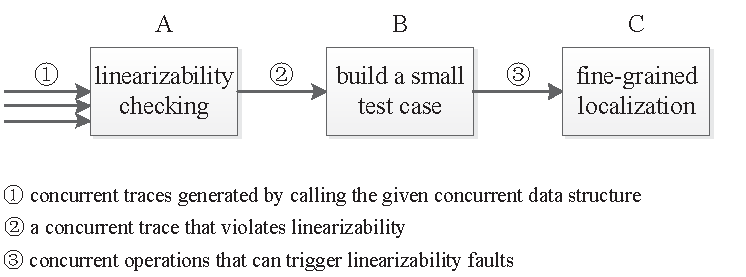
\includegraphics[width = 3.5in]{liucheng.pdf}
\caption{Labels of nodes}\label{fig:liucheng}
\end{figure}

In order to resolve the state space explosion problem, we divide the localization process into a coarse-grained level and a fine-grained level.
The coarse-grained level addresses the issue of working out a test case that contains a small number of operations but is sufficient to trigger a linearizability faults \cite{DBLP:conf/seke/ZhangWZ17}. 
Then, given the small test case as the input
for the fine-grained level localization, the number of memory access instructions that should be investigated 
can be hugely reduced.
Together with a linearizability checking technique \cite{DBLP:journals/concurrency/Lowe17} and coarse-grained localization \cite{DBLP:conf/seke/ZhangWZ17}, the overall process is illustrated as in Fig.\ref{fig:liucheng}, in which C is the main contribution of this work.

Table~\ref{tab:abbreviation} lists the abbreviations that appear frequently throughout the paper.





\begin{table}[]
\centering
\caption{Abbreviations in this paper}
\label{tab:abbreviation}
\begin{tabular}{c|c|c|c|c|c|c|c|c|c}
 CDRS & HLDR & CAS \\
 \textbf{C}ritical \textbf{D}ara \textbf{R}ace \textbf{S}equence& \textbf{H}igh \textbf{L}evel \textbf{D}ata \textbf{R}ace & \textbf{C}ompare \textbf{A}nd \textbf{S}wap \\\hline
 FGVT & CGVT& \\
 \textbf{F}ine-\textbf{G}rained \textbf{V}eri\textbf{T}race &  \textbf{C}oarse-\textbf{G}rained \textbf{V}eri\textbf{T}race & 
\end{tabular}
\end{table}

\noindent\textbf{\textit{Contributions.}}
The contributions of this paper are as follows:
\begin{itemize}
  \item We extend the traditional coarse-grained trace model to a fine-grained trace model by adding memory access events. We also extend the notion of linearizability onto fine-grained traces.
  \item We propose the key notion of \textit{Critical Data Race Sequence} (CDRS) for characterizing the data races that are decisive to linearizability faults.
  \item We develop a labeled interleaving tree model that contains all the possible fine-grained traces of a concurrent execution. Each node corresponds to a data race and is labeled in a way that can reflect the existence of CDRS through a certain pattern.
  \item We implement a prototype tool, \textit{FGVT}, for real-world Java concurrent programs. Experiments show that FGVT is effective, in that all the CDRSes reported by FGVT indeed reveal the root causes of linearizability faults.
\end{itemize}

\noindent\textbf{\textit{Related work.}} Automated linearizability checking algorithms were presented in \cite{DBLP:conf/pldi/BurckhardtDMT10,DBLP:journals/jpdc/WingG93}, but suffered from a bottleneck of performance. Based on \cite{DBLP:journals/jpdc/WingG93}, optimized algorithms were proposed in \cite{DBLP:journals/concurrency/Lowe17} and \cite{DBLP:conf/forte/HornK15a} through partial order reduction and compositional reasoning, respectively. Model checking was applied in \cite{DBLP:conf/popl/BouajjaniEEH15,DBLP:conf/pldi/EmmiEH15} for linearizability checking, with simplified first-order formulas that can help improve efficiency. Fine-grained traces were introduced in \cite{DBLP:conf/sac/LongZ16} to accelerate linearizability checking. All these work lays a firm foundation for the localization of linearizability faults.

Efforts have been devoted to concurrency bug localization, e.g., through an active-testing approach based on bug patterns. The potential bug locations can then be ranked with the suspicious bug patterns gathered. The characteristics of bug patterns were discussed in \cite{DBLP:conf/asplos/LuPSZ08,DBLP:conf/ipps/FarchiNU03} in details. Memory access patterns were proposed in \cite{DBLP:conf/icse/ParkVH10,DBLP:conf/icst/ParkVH12,DBLP:conf/icsm/LiuQWM14} for ranking bug locations. A fault comprehension technique was further presented in \cite{DBLP:conf/icse/Park04} for bug patterns. Definition-use invariants were presented in \cite{DBLP:conf/oopsla/ShiPYLZCZ10} for detecting concurrency bugs with pruning and ranking methods. A constraint-based symbolic analysis method was proposed in \cite{DBLP:conf/issta/KhoshnoodKW15} to diagnose concurrency bugs.

Some other concurrency bug localizations techniques were based on the bug localization techniques for sequential programs. In \cite{DBLP:conf/IEEEpact/GottschlichPPW13}, concurrent predicates were derived from an assertion mechanism to determine whether a data race causes a concurrency bug. Concurrent breakpoints, an adaption of a breakpoint mechanism, were proposed in \cite{DBLP:conf/ppopp/ParkS12} for concurrent program debugging.

We claim that the novelty of this work is that we focus on the correctness criterion of linearizability, and thus tree search also focuses on such a direction. We apply some 
existing tree search techniques such as partial-order reduction but we emphasizes our novel approach of localizing linearizability faults.


\noindent\textbf{\textit{Organization.}} The rest of the paper is organized as follows. Section \ref{sec:motivatingeg} presents an example to illustrate our motivation. Section \ref{sec:fgtracemodel} introduces our fine-grained trace model. Section \ref{sec:criticaldataraces} presents the key notion of CDRS based on our fine-grained trace model. Section \ref{sec:intertree} shows the labeled interleaving tree model, and the pattern of CDRSes. Section \ref{sec:implementation} reports the implementation and experiments about our prototype tool FGVT. Section \ref{sec:conclusion} concludes the paper.

\section{Motivating Example}\label{sec:motivatingeg}

In this section, we illustrate the motivation of this work through a buggy concurrent data structure \textit{PairSnapShot} \cite{DBLP:conf/sac/LongZ16}.

\begin{wrapfigure}[15]{r}{0.55\textwidth}
\centering
    \begin{small}
 \vspace{-0.8cm}
        \begin{verbatim}
    PairSnapShot:
        int d[2];
        write(i,v){
            d[i] = v;                #1
        }
        Pair read(){
            while(true){
                int x = d[0];        #2
                int y = d[1];        #3
                if(x == d[0])        #4
                    return <x,y>;
            }
        }
        \end{verbatim}
        \vspace{-1cm}
        \end{small}
        \caption{A concurrent data structure: PairSnapShot}
        \label{fig:pairsnapshot}
\end{wrapfigure}


Fig.\ref{fig:pairsnapshot} shows a simplified version of PairSnapShot, where it holds an array \texttt{d} of size 2. A \texttt{write(i,v)} operation writes \texttt{v} to \texttt{d[i]}, while a \texttt{read} \texttt{$\to \langle v_0,v_1\rangle$} operation reads the values of \texttt{d[0]} and \texttt{d[1]}, which are $v_0$ and $v_1$, respectively.

 A correctness criterion of PairSnapShot is that \texttt{read} should always return the values of the same moment. However, 
Fig.~\ref{fig:psscoarsetrace} shows a concurrent execution in which the return values of \texttt{read} do not exist at any moment of the execution. 
In Fig.~\ref{fig:psscoarsetrace}, time moves from left to right; dark lines indicate the time intervals of operations and  
the short vertical lines at the both ends of a dark line represent the moment when an operation is invoked and returned, respectively.
A label ${t:(v_0,v_1)}$ indicates that at the moment $t$,  \texttt{d[0]} is $v_0$ and \texttt{d[1]} is $v_1$.
  The operation \texttt{read()} on Thread 2 returns a value $\mathtt{\pair{1,2}}$,
  which is not consistent with value of any moment. 
  %The `\texttt{x}' labels in Fig.\ref{fig:pairsnapshot} mark the moments when each instruction takes effects, which explains exactly the cause of the linearizability fault.

The reason of this violation can be found out by enumerating the possible executing orders of memory access events which is labeled by \texttt{\#} in Fig.~\ref{fig:pairsnapshot}. 
One possible order that can trigger the violation is illustrated in Fig.~\ref{fig:pssfinetrace}, in which ``\texttt{x}'' indicate the executing moments of the corresponding memory access events. 
Actually, this model checking approach is the most common way to locate the root cause of concurrency bugs, and has been studied in many existing literatures.
Here, our focus is not on how to find this fine-grained executing order, but to study how the thread execution order, which causes data race, influences the final result of linearizability.

%The fine-grained root cause can be explained by the temporal order of instructions labeled by ``\texttt{x}''. Since \texttt{d[0]} and \texttt{d[1]} should be considered as a whole (a pair), instructions in \texttt{write} and \texttt{read} should accordingly be considered accessing the whole pair, and thus data races exist there. In this execution, all data races between instructions of \texttt{write} and \texttt{read} together result in the linearizability fault, and all ones are necessary to trigger the linearizability fault.



\begin{figure}[!ht]
\centering
\setlength{\unitlength}{0.8cm}
\begin{picture}(10,2.5)
\thinlines

\multiput(1.7,1.5)(0.2,0){44}{\line(1,0){0.1}}
\thicklines
\put(2.0,1.5){\line(1,0){1.7}}
\put(4.1,1.5){\line(1,0){1.7}}
\put(6.2,1.5){\line(1,0){1.7}}
\put(8.3,1.5){\line(1,0){1.7}}
\begin{small}
\put(0,1.4){Thread 1}
\put(1.9,1.7){$\mathtt{write(0,2)}$}
\put(4.0,1.7){$\mathtt{write(1,2)}$}
\put(6.1,1.7){$\mathtt{write(1,1)}$}
\put(8.2,1.7){$\mathtt{write(0,1)}$}
\put(0,0.4){Thread 2}

\put(1.0,2.3){$t_1:\pair{1,1}$}
\put(3.0,2.3){$t_2:\pair{2,1}$}
\put(5.0,2.3){$t_3:\pair{2,2}$}
\put(7.1,2.3){$t_4:\pair{2,1}$}
\put(9.2,2.3){$t_5:\pair{1,1}$}

\thinlines

\multiput(1.7,0.5)(0.2,0){44}{\line(1,0){0.1}}
\thicklines
\put(2.3,0.5){\line(1,0){7.5}}
\put(4.6,0.7){\color{red}{$\mathtt{read\to \pair{1,2}}$}}

\put(2.3,0.4){\line(0,1){0.2}}
\put(9.8,0.4){\line(0,1){0.2}}

\put(2.0,1.4){\line(0,1){0.2}}
\put(4.1,1.4){\line(0,1){0.2}}
\put(6.2,1.4){\line(0,1){0.2}}
\put(8.3,1.4){\line(0,1){0.2}}

\put(3.7,1.4){\line(0,1){0.2}}
\put(5.8,1.4){\line(0,1){0.2}}
\put(7.9,1.4){\line(0,1){0.2}}
\put(10,1.4){\line(0,1){0.2}}

\thinlines
\multiput(1.8,0.3)(0,0.2){10}{\line(0,1){0.1}}
\multiput(3.9,0.3)(0,0.2){10}{\line(0,1){0.1}}
\multiput(6.0,0.3)(0,0.2){10}{\line(0,1){0.1}}
\multiput(8.1,0.3)(0,0.2){10}{\line(0,1){0.1}}
\multiput(10.2,0.3)(0,0.2){10}{\line(0,1){0.1}}





\end{small}
\end{picture}
\caption{A buggy trace of PairSnapShot}
\label{fig:psscoarsetrace}
\end{figure}


\vspace{-1cm}

\begin{figure}[!ht]
\centering
\setlength{\unitlength}{0.8cm}
\begin{picture}(10,2.5)
\thinlines

\multiput(1.7,1.5)(0.2,0){44}{\line(1,0){0.1}}

\begin{small}
\put(0,1.4){Thread 1}

\put(0,0.4){Thread 2}

\put(1.0,2.3){$t_1:\pair{1,1}$}
\put(3.0,2.3){$t_2:\pair{2,1}$}
\put(5.0,2.3){$t_3:\pair{2,2}$}
\put(7.1,2.3){$t_4:\pair{2,1}$}
\put(9.2,2.3){$t_5:\pair{1,1}$}

\thinlines

\multiput(1.7,0.5)(0.2,0){44}{\line(1,0){0.1}}





\thinlines
\multiput(1.8,0.3)(0,0.2){10}{\line(0,1){0.1}}
\multiput(3.9,0.3)(0,0.2){10}{\line(0,1){0.1}}
\multiput(6.0,0.3)(0,0.2){10}{\line(0,1){0.1}}
\multiput(8.1,0.3)(0,0.2){10}{\line(0,1){0.1}}
\multiput(10.2,0.3)(0,0.2){10}{\line(0,1){0.1}}




\put(3.0,1.4){\texttt{x}}
\put(4.6,1.4){\texttt{x}}
\put(6.6,1.4){\texttt{x}}
\put(8.8,1.4){\texttt{x}}

\put(2.7,0.4){\texttt{x}}
\put(5.4,0.4){\texttt{x}}
\put(9.3,0.4){\texttt{x}}



\put(2.3,0.4){\line(0,1){0.2}}
\put(9.8,0.4){\line(0,1){0.2}}

\put(2.0,1.4){\line(0,1){0.2}}
\put(4.1,1.4){\line(0,1){0.2}}
\put(6.2,1.4){\line(0,1){0.2}}
\put(8.3,1.4){\line(0,1){0.2}}

\put(3.7,1.4){\line(0,1){0.2}}
\put(5.8,1.4){\line(0,1){0.2}}
\put(7.9,1.4){\line(0,1){0.2}}
\put(10,1.4){\line(0,1){0.2}}

\put(2.1,0.1){$c_r$}
\put(9.8,0.1){$r_r$}

\end{small}
\begin{scriptsize}

\put(2.9,1.1){\texttt{\#1}}
\put(4.6,1.1){\texttt{\#1}}
\put(6.6,1.1){\texttt{\#1}}
\put(8.8,1.1){\texttt{\#1}}

\put(2.7,0.1){\texttt{\#2}}
\put(5.4,0.1){\texttt{\#3}}
\put(9.3,0.1){\texttt{\#4}}

\put(2.0,1.1){$c_{w1}$}
\put(4.0,1.1){$c_{w2}$}
\put(6.0,1.1){$c_{w3}$}
\put(8.1,1.1){$c_{w4}$}

\put(3.4,1.1){$r_{w1}$}
\put(5.4,1.1){$r_{w2}$}
\put(7.5,1.1){$r_{w3}$}
\put(9.6,1.1){$r_{w4}$}
\end{scriptsize}

\end{picture}
\caption{An executing order of memory access events triggering the violation in Fig.~{\ref{fig:psscoarsetrace}}}
\label{fig:pssfinetrace}
\end{figure}





\section{Preliminary}\label{sec:fgtracemodel}


In this section, we extend the traditional coarse-grained trace model \cite{DBLP:conf/popl/BouajjaniEEH15}, recalled in Section \ref{sec:coarsegraintm}, to the fine-grained trace model presented in Section \ref{sec:finegraintm}. Compared to the traditional one, our new model includes memory access instructions such as \texttt{read, write} and atomic primitive \textit{compare-and-swap} (\texttt{CAS}). This enables us to reason about the causes of linearizability faults on the fine-grained level.

\subsection{Coarse-grained trace model}\label{sec:coarsegraintm}
A \textit{trace} $S$ is a finite sequence of events $e(\mathit{Arg})^{\left\langle o,t\right\rangle}$, where $e$ is an event symbol ranging over a pre-defined set $E$, $\mathit{Arg}$ represents the list of arguments, $o$ belongs to a set $O$ of operation identifiers and $t$ belongs to a set $T$ of thread identifiers. In the coarse-grained trace model, the set $E$ contains the following subsets:
\begin{itemize}
  \item $\ecall$ contains symbols that represent operation invocation events. An invocation event is represented as $c(v_a)^{\langle o,t\rangle}$ $(c\in \ecall)$, where $v_a$ is the argument of the operation;
  \item $\eresp$ contains symbols that represent operation response events. A response event is represented as $r(v_r)^{\langle o,t\rangle}$ $(r\in \eresp)$, where $v_r$ is the return value of the operation.
\end{itemize}
\noindent In this paper we also use $\ecall, \eresp$ to represent the set of the corresponding events indiscriminately, and symbol $e\in \ecall\cup \eresp$ to represent an event. The order relation between events in a trace $S$ is written as $\prec_S$ (or $\prec$), i.e., $e_1\prec_S e_2$ if $e_1$ is ordered before $e_2$ in $S$. We denote the operation identifier of an event $e$ as $\mathtt{op}(e)$, and thread identifier as $\mathtt{td}(e)$. An invocation event $c\in \ecall$ and a response event $r\in \eresp$ \textit{match} if $\mathtt{op}(c) = \mathtt{op}(r)$, written as $c\diamond r$. A pair of matching events forms an operation instance with an operation identifier in $O$, and we usually represent an operation as $m(v_a)\to v_r$, where $m$ is the operation name.
 
 A trace $S = e_1e_2\cdots e_n$ is \textit{well-formed} if it satisfies that:
\begin{itemize}
  \item Each response is preceded by a matching invocation:\\
  $e_j\in \eresp$ implies $e_i \diamond e_j$ for some $i<j$
  \item Each operation identifier is used in at most one invocation/response:\\
  $\mathtt{op}(e_i)=\mathtt{op}(e_j)$ and $i<j$ implies $e_i \diamond e_j$
\end{itemize}
 A well-formed trace $S$ can also be treated as a partial order set $\pair{S,\sqsubset_S}$ of operations on \textit{happen-before} relation $\sqsubset_S$ between operations, where $S$ is called a \textit{coarse-grained trace} (or \textit{coarse-grained history}). The \textit{happen-before} relation $\sqsubset_S$ is defined as that: assuming two operations $O_1,O_2$ in $S$ are formed by $c_1,r_1$ and $c_2,r_2$ respectively, then $O_1\sqsubset_S O_2$ if and only if $r_1\prec c_2$.

\begin{example}
Fig.~\ref{fig:psscoarsetrace} shows such a well-formed trace:
$S = c_{w1}c_rr_{w1}c_{w2}r_{w2}c_{w3}r_{w3}c_{w4}r_{r}r_{w4}$, where $c_{wi}$ and $r_{wi}$
represents the invocation and response events of the $i$-th $\mathtt{write}$ operation respectively, and
$c_r$ and $r_r$ represent the invocation and response events of the $\mathtt{read}$ operation.

In this example, it is obvious that \begin{small}$\wri(0,2)\prec \wri(1,2)\prec \wri(1,1)\prec \wri(0,1)$\end{small}, 
but there is no \hb  
relation between the $\rea$ operation and any of the $\wri$ operations.

\end{example}




A coarse-grained trace $S$ is \textit{sequential} if $\sqsubset_S$ is a total order. 
We define that a \textit{specification} of an object is the set of all sequential traces that satisfy the correctness criteria of that object. 
Note that here correctness criterion is specified by concurrent data structures, such as \textit{first-in-first-out} rule for \textit{FIFO-Queue}, \textit{first-in-last-out} rule for \textit{Stack}.

\begin{myDef}[Linearizability]\label{def:linearizability}
A coarse-grained trace $S$ of an object is linearizable if there exists a sequential trace $S'$ in the specification of the object such that:
\begin{enumerate}
  \item $S = S'$, i.e., operations in $S$ and $S'$ are the same;
  \item $\sqsubset_S \subseteq \sqsubset_{S'}$, i.e., given two operations $O_1$, $O_2$ in $S$, $S'$, if $O_1\sqsubset_S O_2$, then $O_1\sqsubset_{S'} O_2$.
\end{enumerate}
\end{myDef}

Note that this definition speaks only complete traces, neglecting the existence of pending operations, that is, the operations without response events. Since this paper focuses on analysis of linearizability faults rather than detection, we consider complete traces only.

\begin{example}
Fig.~\ref{fig:accounttwoseqtraces} shows 5 sequential traces that satisfy requirements 1 and 2 in Definition \ref{def:linearizability} with respect to the coarse-grained trace shown in Fig~\ref{fig:psscoarsetrace}. However, neither of them satisfies the correctness criteria of \textit{PairSnapShot}, by which the $\mathtt{read}$ operation should not return $\pair{1,2}$, so that neither of them belongs to the specification set of \textit{PairSnapShot}. Therefore we can say that the coarse-grained trace in Fig.~\ref{fig:psscoarsetrace} is non-linearizable.

\end{example}

\begin{figure}
\centering
\setlength{\unitlength}{0.5cm}
    \begin{picture}(17.5,5)
    \begin{footnotesize}
	\put(0,4.5){$1: \mathtt{read\to \pair{1,2}}$\quad $\mathtt{write(0,2)}$\quad $\mathtt{write(1,2)}$ \quad$\mathtt{write(1,1)}$\quad $\mathtt{write(0,1)}$}
	
	\put(0,3.5){$2: \mathtt{write(0,2)}$\quad $\mathtt{read\to \pair{1,2}}$\quad $\mathtt{write(1,2)}$\quad $\mathtt{write(1,1)}$\quad $\mathtt{write(0,1)}$}
	
	\put(0,2.5){$3: \mathtt{write(0,2)}$\quad $\mathtt{write(1,2)}$ \quad$\mathtt{read\to \pair{1,2}}$\quad  $\mathtt{write(1,1)}$\quad $\mathtt{write(0,1)}$}
	
	\put(0,1.5){$4: \mathtt{write(0,2)}$\quad $\mathtt{write(1,2)}$ \quad$\mathtt{write(1,1)}$ \quad$\mathtt{read\to \pair{1,2}}$\quad $\mathtt{write(0,1)}$}
	
	\put(0,0.5){$5: \mathtt{write(0,2)}$\quad $\mathtt{write(1,2)}$ \quad$\mathtt{write(1,1)}$\quad $\mathtt{write(0,1)}$ \quad$\mathtt{read\to \pair{1,2}}$}
	\end{footnotesize}
    \end{picture}

    \caption{Five possible sequential traces}\label{fig:accounttwoseqtraces}
\end{figure}

\subsection{Fine-grained trace model}\label{sec:finegraintm}


In the fine-grained trace model,  the symbol set $E$ has other subsets of events in addition to $\ecall$ and $\eresp$:

\begin{itemize}
  \item $\ewrite$ contains symbols that represent the \textit{memory writing} events. An event of memory writing is represented as $wr(addr,v)^{\left\langle o,t\right\rangle}$ $(wr \in \ewrite)$, where $addr$ is the memory location to be modified to a value $v$;
  \item $\eread$ contains symbols that represent the \textit{memory reading} events. An event of memory reading is represented as $rd(addr)^{\left\langle o,t\right\rangle}$ $(rd \in \eread)$, where $addr$ is the memory location to be read;
  \item $\ecas$ contains symbols that represent the \textit{atomic primitive}, such as \textit{compare-and-swap} (\textit{CAS}) in modern architecture. A \textit{CAS} event can be represented as $cas(addr, v_e, v_n)^{\left\langle o,t\right\rangle}$ $(cas \in \ecas)$, where $addr$ represents a memory location, $v_e$ and $v_n$ are two values. The function of this atomic primitive is that if the value at $addr$ equals to $v_e$, it will be updated to $v_n$ and return $\mathtt{true}$, otherwise it would not do anything but return $\mathtt{false}$.
  %\item $\mathsf{OAI}$ contains symbols that represent other atomic instructions, such as \textit{double-compare-and-swap} (\textit{DCAS}). All these events can be represented as $oai(Arg)^{\left\langle o,t\right\rangle}$ $oai\in \mathsf{OAI}$
\end{itemize}
\noindent Similarly, in this paper $\ewrite, \eread, \ecas$ also represent the corresponding sets of events. Let $\mathsf{M} = \ewrite\cup\eread\cup\ecas$, events $e$ such that $e\in \mathsf{M}$ are called \textit{memory access events}.


A fine-grained trace $S_f$ is a total order set $\pair{S_f,\prec}$ of events over set $E= \ecall\cup \eresp\cup \ewrite\cup \eread\cup \ecas $.
%We define a prefix of a fine-grained trace $S_f$ ending with an event $e'$ as the subset of $S_f$ containing all events $e$ such that $(e\prec e')\vee (e=e')$, written as $\mathtt{P}_{S_f}(e')$.
We define a projection $\mathcal{F}_{c}$ that maps a fine-grained trace $S_f$ to a coarse-grained trace $S_c$ by dropping all memory access events in $S_f$, i.e., $ \mathcal{F}_c(S_f) = S_f|_{\{\ecall,\eresp\} }$. A fine-grained trace $S_f$ is \textit{well-formed} if it satisfies that:

\todo{this definition is not clear}

\begin{itemize}
  \item $\mathcal{F}_c(S_f)$ is well-formed;
  \item The operation identifier of any memory access event in $S_f$ is consistent with that of one pair of  matching invocation/response events  in $S_f$, i.e.,
  %For any memory access event in $S_f$, its operation identifier is one that occurs in an invocation/response event in $\mathcal{F}_c(S_f)$, i.e., 
      $\forall e_m\exists e_o.(\mathtt{op}(e_m)= \mathtt{op}(e_o))$, where $e_m$ is a memory access event and $e_o$ is either of a pair of matching invocation/response events in $S_f$.
  \item All memory access events with operation identifier $o$ lie between the consistent matching invocation/response event pair with the operation identifier $o$, i.e.,
      $\forall e.((\mathtt{op}(e)=o)\to(c\prec e\prec r))$, where $e$ is a memory access event in $S_f$, and $c,r$ are matching invocation and response events with thread identifier $o$.
  %For any matching events $c\in \ecall$ and $r\in \eresp$ such that $\mathtt{op}(c)=\mathtt{op}(r)=o$, then: \\ $\forall e\in \mathsf{M}.( \mathtt{op}(e) = o \longrightarrow c\prec e \prec r)$.
\end{itemize}
\noindent We claim that all fine-grained traces in this paper are well-formed.

%\begin{figure}
\begin{subfigure}[b]{0.24\textwidth}
    \setlength{\unitlength}{0.5cm}
    \begin{picture}(6.5,2.6)
        \begin{small}
        \put(0,1.7){Thd 1}
        \put(0,0.4){Thd 2}
        \end{small}
        \thinlines
        \multiput(2,1.8)(0.2,0){27}{\line(1,0){0.1}}
        \multiput(2,0.5)(0.2,0){27}{\line(1,0){0.1}}

        \thicklines
        \put(2.3,1.8){\line(1,0){3}}
        \put(3.2,0.5){\line(1,0){3}}

        \put(2.3,1.7){\line(0,1){0.2}}
        \put(3.2,0.4){\line(0,1){0.2}}
        \put(5.3,1.7){\line(0,1){0.2}}
        \put(6.2,0.4){\line(0,1){0.2}}



        \put(2.2,2.1){$c_1$}
        \put(5.2,2.1){$r_1$}
        \put(2.8,0.8){$c_2$}
        \put(5.8,0.8){$r_2$}

        \put(3.7,2.1){$O_1$}
        \put(4.2,0.8){$O_2$}
    \end{picture}
    \caption{A coarse-grained trace}\label{fig:coarsegrainedtrace}
\end{subfigure}
\hfill
\begin{subfigure}[b]{0.24\textwidth}
    \setlength{\unitlength}{0.5cm}
    \begin{picture}(6.5,2.6)
        \begin{small}
        \put(0,1.7){Thd 1}
        \put(0,0.4){Thd 2}
        \end{small}
        \thinlines
        \multiput(2,1.8)(0.2,0){27}{\line(1,0){0.1}}
        \multiput(2,0.5)(0.2,0){27}{\line(1,0){0.1}}

        \thicklines
        \put(2.3,1.8){\line(1,0){3}}
        \put(3.2,0.5){\line(1,0){3}}

        \put(2.3,1.7){\line(0,1){0.2}}
        \put(3.2,0.4){\line(0,1){0.2}}
        \put(5.3,1.7){\line(0,1){0.2}}
        \put(6.2,0.4){\line(0,1){0.2}}



        \put(2.2,2.1){$c_1$}
        \put(5.2,2.1){$r_1$}
        \put(2.8,0.8){$c_2$}
        \put(5.8,0.8){$r_2$}

        \put(3.7,2.1){$O_1$}
        \put(4.2,0.8){$O_2$}
    \end{picture}
    \caption{A coarse-grained trace}\label{fig:coarsegrainedtrace2}
\end{subfigure}

\end{figure}



\begin{example}
Fig.\ref{fig:pssfinetrace} presents a well-formed fine-grained trace:\\
 \quad\quad\quad\quad$S_f = c_{w1}c_r$\texttt{\#2\#1}$r_{w1}c_{w2}$\texttt{\#1\#3}$r_{w2}c_{w3}$\texttt{\#1}$r_{w3}c_{w4}$\texttt{\#1\#4}$r_{r}r_{w4}$\\
and the $\prec$ relations between events are obvious. 
Application of $\mathcal{F}_{c}$ to this fine-grained trace results in the coarse-grained trace in Fig.\ref{fig:psscoarsetrace}.
\end{example}

\begin{myDef}
The linearizability of $S_f$ depends on the linearizability of $\mathcal{F}_c(S_f)$, i.e., if $\mathcal{F}_c(S_f)$ is linearizable, then $S_f$ is linearizable. \end{myDef}

We define a predicate $\mathcal{L}_n$ to denote the linearizability of $S_f$, i.e., if $S_f$ is linearizable, then $\mathcal{L}_n(S_f)$ is true.


\section{Critical Data Race Sequence}\label{sec:criticaldataraces}



In this section, we analyze linearizability faults on the fine-grained level, and propose \textit{critical data race sequence} (\textit{CDRS}) which exposes the root cause of linearizability faults.



%Given a coarse-grained trace $S_c$, we define a set $\mathbb{U}$ of fine-grained traces such that all fine-grained traces $S_f$ in $\mathbb{U}$ can be mapped by $\mathcal{F}_c$ to a coarse-grained trace $S'_c$ satisfying that:
%\begin{itemize}
%  \item $S'_c$ and $S_c$ have the same elements;
%  \item $\sqsubset_{S_c}\subseteq \sqsubset_{S'_c}$, i.e., $S'_c$ holds the \textit{happen-before} relation in $S_c$.
%\end{itemize}
%\noindent Actually, a $\mathbb{U}$ corresponds to a concurrent program whose execution can produce $S_c$, and all possible fine-grained traces resulting from the concurrent program are maintained in $\mathbb{U}$.
\begin{myDef}[Concurrent program]\label{def:concurrentprogram}
%Given a coarse-grained trace $S_c$, we define the \textit{concurrent program} that results in $S_c$ as a set $\mathbb{P}$ of fine-grained traces. Each fine-grained trace $S_f\in \mathbb{P}$ can be mapped by $\mathtt{F_c}$ to a coarse-grained trace $S'_c$, and each $S'_c$ should satisfy that:
Given a coarse-grained trace $\ct$, we define a concurrent program $\p$:
%Let \ct be a coarse-grained trace.
%\ct corresponds to a concurrent program \p.
$\p$ 
 is a set of fine-grained traces such that
every fine-grained trace $\ft \in \p$ can be mapped to a coarse-grained trace $S'_c$, which satisfies that: 
 %such that each coarse-grained trace $S'_c=\mathtt{F_c}(S_f)$ mapped from each fine-grained trace $S_f\in \mathbb{P}$ satisfies that:
\begin{itemize}
  \item $S'_c = S_c$, i.e., operations in $S'_c$ and $S_c$ are the same;
  \item $\sqsubset_{S_c}\subseteq \sqsubset_{S'_c}$, i.e., $S'_c$ preserves the \textit{happen-before} relation in $S_c$.
\end{itemize}
\end{myDef}

%\noindent \textbf{Example}
%Fig.1(c) can be considered as a $\mathbb{P}$ derived from Fig.1(a), and all fine-grained traces $S_f$ such that $\mathcal{F}_c(S_f)$ results in sequential trace $O_1O_2$, $O_2O_1$ or concurrent trace in Fig.1(a) are maintained in this $\mathbb{P}$. It can also be considered as a program whose executions can result in those fine-grained traces.
Intuitively, a program $\mathbb{P}$ maintains all %possible 
fine-grained traces that preserve the \textit{happen-before} relation of $S_c$.
%after an application of $\mathtt{F_c}$. 
If $S_c$ is sequential, then we say the program $\p$ w.r.t. $\ct$ is sequential.
And, if there exists a non-linearizable fine-grained trace in a program $\p$, we say that $\p$ is non-linearizable.

\begin{myDef}[Linearizability fault]
Let $\p$ be a non-linearizable concurrent program. A \textit{linearizability fault} $\mathcal{F}$ is defined as a non-linearizable fine-grained trace $S_f$ in $\p$.
\end{myDef}

%Since a fine-grained trace is a total order of events, we can define a prefix relation $\subseteq_{pre}$ between two fine-grained traces, 
We define the prefix relation $\subseteq_{pre}$ between two fine-grained trace $S_1$ and $S_2$, that is, $S_1\subseteq_{pre} S_2$ says that $S_1$ is a prefix of $S_2$. We use $\cdot$ to represent the concatenation of a sequence of events and another sequence of events, that is, if $S_1=e_1\cdots e_n$ and $S_2 = e_{n+1}\cdots e_{n+m}$, then $S_1\cdot S_2 = e_1\cdots e_n e_{n+1}\cdots e_{n+m}$.

\begin{myDef}[High-level data race \cite{DBLP:journals/stvr/ArthoHB03}]\label{def:datarace}
Let $\p$ be a concurrent program. 
A \textit{high-level data race} (\textit{HLDR}) $\mathsf{D}$ in $\mathbb{P}$ is defined as a triple $\left\langle \mathit{Var}, \se, \ce\right\rangle$. 
Here, $\mathit{Var}$ is a set of one or more shared variables, each corresponding to a memory location. $\se$ is a sequence of events.
%and the execution of $\se$ leads $\mathit{Var}$ to an initial state.
%which can give $\mathit{Var}$ an initial state by executing the sequence of events. 
%$\se$ is also a prefix of some traces in $\mathbb{P}$. 
$\ce$ is a set of two or more memory access events $e(\mathit{Arg})^{\left\langle o,t\right\rangle}$, such that:

\begin{itemize}
\item each event $e$ has a distinct thread identifier $o$;
\item each event $e$ accesses some shared variables in $\mathit{Var}$;
\item no temporal relation between each pair of the events;
\item for any permutation $S_p$ of events in $\ce$, there exists a fine-grained trace $S\in \p$ such that $\se \cdot S_p \subseteq_{pre} S$.
\end{itemize}
%$\ce$ satisfies that:

%$$ \forall P  \exists S (\se\cdot P\subseteq_{pre} S)$$

%\noindent where $P$ is a permutation of events in $\ce$, and $S$ is a fine-grained trace in $\mathbb{P}$.


\end{myDef}

Note that here the decision of $\mathit{Var}$ depends on the algorithm of the shared object. The most common situation is that several events 
simultaneously access the same memory location and do some read or modification. 
However, there also exist other situations, such as \textit{PairSnapShot} in Section \ref{sec:motivatingeg}, in which case several memory locations should be considered as a whole.

Given a HLDR $\mathsf{D}  = \left\langle \mathit{Var}, \se, \ce\right\rangle$ where $e_1, e_2\in \ce$, we say $e_1$ \textit{wins} $e_2$ with respect to a fine-grained trace $S_f$ if 
 $\se\cdot e_1e_2 \subseteq S_f $.
 
 Given a $\mathbb{P}$, we define a partial order relation $<_{dr}$ between two HLDRs $\mathsf{D}_1=\left\langle \mathit{Var}_1, \se_1, \ce_1\right\rangle$ and $\mathsf{D}_2 = \left\langle \mathit{Var}_2, \se_2, \ce_2\right\rangle$, that is, if $\se_1\subseteq_{pre}\se_2$, then $\mathsf{D}_1<_{dr}\mathsf{D}_2$. 




\begin{myTheo}\label{theo:datarace}
   If there is a linearizability fault, then there is a high-level data race.
\end{myTheo}

\begin{proof}
To prove Theorem \ref{theo:datarace}, it suffices to prove the contrapositive proposition that if there is no high-level data race, 
then there is no linearizability fault. According to Definition \ref{def:datarace}, the premise, no high-level data race, means that in $\ce$:

$$\exists S_p \forall S ( \se\cdot S_p \nsubseteq_{pre} S)$$

Here, if $\mathbb{P}$ is a concurrent program, this condition is not satisfied according to Definition \ref{def:concurrentprogram}. 
Therefore, the $\mathbb{P}$ that satisfies this condition corresponds to a sequential program, and the sequential trace surely has no linearizability fault.
\end{proof}


\begin{myDef}[Critical data race sequence]\label{def:cdrs}
    Let  $\mathbb{P}$ be a concurrent program, $\mathcal{F}$ be a linearizability fault. A \textit{Critical Data Race Sequence} (\textit{CDRS}) with respect to
 $\mathcal{F}$ is a total order set of data races $\{\mathsf{D}_1,\mathsf{D}_2,\cdots,\mathsf{D}_n\}$
 \[
\begin{array}{ccc}
   \{& \langle\mathit{Var}_1, \se_1, \ce_1 = \set{e_{11},e_{12},\cdots,e_{1m_1}}\rangle, & \\
   & \langle\mathit{Var}_2, \se_2, \ce_2 = \set{e_{21},e_{22},\cdots,e_{2m_2}}\rangle, &\\
   & \vdots& \\
   &\langle \mathit{Var}_n, \se_n, \ce_n = \set{e_{n1},e_{n2},\cdots,e_{nm_n}} \rangle&\}
\end{array}
\]

\noindent where the relation $<_{dr}$ exists as $\mathsf{D}_1 <_{dr} \dr_2 <_{dr} \cdots  <_{dr} \mathsf{D}_n$.
A CDRS satisfies that there exist two events $e_{i1}, e_{i2}\in \ce_i$ ($i\in{1,\dots,n}$)   that $e_{i1}$'s win and
$e_{i2}$'s win lead the program to ``inverse'' consequences. Here the meaning of ``inverse'' includes that
\begin{itemize}
\item If all the fine-grained traces $S_{f1}$ such that $\se\cdot e_{i1} \subseteq_{pre}$ are linearizable, then there exist fine-grained traces $S_{f2}$ such that 
$\mathit{SE_i}\cdot e_{i2}$ that are non-linearizable;
\item If all the fine-grained traces $S_{f1}$ such that $\se\cdot e_{i1} \subseteq_{pre}$ are non-linearizable, then there exist fine-grained traces $S_{f2}$ such that 
$\mathit{SE_i}\cdot e_{i2}$ that are linearizable.\\
\end{itemize}
\end{myDef}


Intuitively, a \textit{CDRS} contains all the HLDRs which are decisive to the linearizability of the trace. Note that although different \textit{CDRS}es in a program $\mathbb{P}$ may lead to different linearizability faults, what we focus on is just the linearizability of the trace and thus we consider all linearizability faults identical in terms of the aspect to lead the trace non-linearizable.

\begin{example} 

Take a look at the example of a HLDR $\mathsf{D}  = \left\langle \mathit{Var}, \se, \ce\right\rangle$  in \textit{PairSnapShot} in which $\ce = \{$\texttt{\#1,\#2}$\}$. If \texttt{\#1} wins, then a non-linearizable trace will never occur; but if \texttt{\#2} like Fig.~\ref{fig:pssfinetrace}, there exists at least such a fine-grained trace that is non-linearizable. In this sense,  $\mathsf{D}$ is included in a CDRS with respect to the linearizability fault $\mathcal{F}$ shown in Fig.~\ref{fig:pssfinetrace}.

\end{example}

\section{Identify CDRS on Interleaving Tree}\label{sec:intertree}
From Section \ref{sec:criticaldataraces}, we know that it is the competitions happening in \textit{CDRS}es that trigger the linearizability faults. In order to identify \textit{CDRS}, we propose an approach based on a model called labeled interleaving tree in this section. Firstly, we represent the fine-grained traces in an interleaving tree, and then we label the nodes of the tree with a symbol system. We will show that all \textit{CDRS}es follow a certain pattern and thus we can identify them based on the characteristics of nodes. 
\subsection{Interleaving tree}

Firstly, we define a projection $\mathtt{F_M}$ mapping a fine-grained trace $S_f$ to a trace $S^M_f$ composed of only memory access events in $S_f$, i.e., $\mathtt{F_M}(S_f) = S_f|_{\mathsf{M}}$. Surely the linearizability of $S^M_f$ is consistent with that of $S_f$.  Besides, we define a state, written as $\mathit{State}$, of an object to be a projection mapping memory locations to their values.

\begin{myDef}[Interleaving Tree]
    An \textit{Interleaving Tree} of $\mathbb{P}$ is a tree, where each node corresponds to a state, and each edge corresponds to a memory access event. A subtree rooted at node $N_d$ is represented as $\mathcal{T}ree(N_d)$. The set of the leaves of the tree is represented as $N_{lf}$.
\end{myDef}

    Algorithm \ref{algo:forminttree} presents how to build an interleaving tree recursively. In line 1, $State$ is initiated to the initial state of the object. The set $\mathit{enS}$ in line 2 initially contains the events which are minimal w.r.t. $\prec$ over the events with the same thread identifier, and thus the number of elements in $\mathit{enS}$ is the same as the number of threads. Line 3-11 is the process of building tree. Firstly, a node is built as line 4 shows. Then, events in $\mathit{enS}$ are traversed, each accessing a memory location $addr$ as line 5 shows. When an event is accessed, a corresponding edge is built as in line 6. Then the state is updated by substituting the value of $addr$ with $v_n$ as in line 7. Here note that if $e$ is an $\eread$ event, $State$ will not be modified. And $\mathit{enS}$ is updated as line 8 shows, where $e$ will be replaced by its successor w.r.t. $\prec$ over the events with the same thread identifier. Finally, the updated $\mathit{State}$ and $\mathit{enS}$ are applied as arguments to another invocation of \textsc{BuildTree} as line 9 shows to build a subtree recursively.



\begin{algorithm}
    \caption{Building of Interleaving Tree}\label{algo:forminttree}
    \begin{algorithmic}[1]
        \State $\mathit{State} = \mathit{State}_{init}$
        \State $\mathit{enS} = \left\{ e | \forall \epsilon\in \mathsf{M} .(\mathtt{td}(\epsilon)=\mathtt{td}(e)\longrightarrow e\prec \epsilon)\right\}$
        \Function{BuildTree}{$\mathit{State},\mathit{enS}$}
            \State \Call{New Node}{$\mathit{State}$}
            \For{$e(addr,v_n)^{\pair{o,t}} \leftarrow \mathit{enS}$}
                \State \Call{New Edge}{$e$}
                \State $\mathit{State} \gets \mathit{State[v_n/addr]}$
                \State $\mathit{enS} \gets \mathit{enS}\setminus \set{e} \cup \set{e'}$
                \State \Call{BuildTree}{$\mathit{State},\mathit{enS}$}
            \EndFor
        \EndFunction
    \end{algorithmic}
\end{algorithm}

\begin{example} 
According to Algorithm \ref{algo:forminttree}, we build the interleaving tree of the concurrent program $\mathbb{P}$ corresponding to Fig.\ref{fig:psscoarsetrace} and present it in Fig.\ref{fig:interleavingtreeofpairsnapshot}. Each node represents a state, and each edge represents a memory access event.

Although due to the limitation of space we have omitted many paths, we can still see that this tree maintains all the fine-grained traces in $\mathbb{P}$, and among these traces the one with bold paths corresponds to 
the non-linearizability situation in Fig.\ref{fig:pssfinetrace}.
\end{example}






\subsection{Identify CDRS on labeled interleaving tree}\label{sec:identifycdrs}
After building an interleaving tree, we design a symbol system to label the tree in order for the identification of CDRS.



Since each leaf $l_f\in N_{lf}$ corresponds to a fine-grained trace from root to itself, we directly apply $\mathcal{L}_n$ to $l_f$ to check the linearizability of the corresponding fine-grained trace. Here, we take a binary interleaving tree built by traces with two threads to illustrate our symbol system.

\begin{wrapfigure}[18]{c}{0.6\textwidth}
\centering
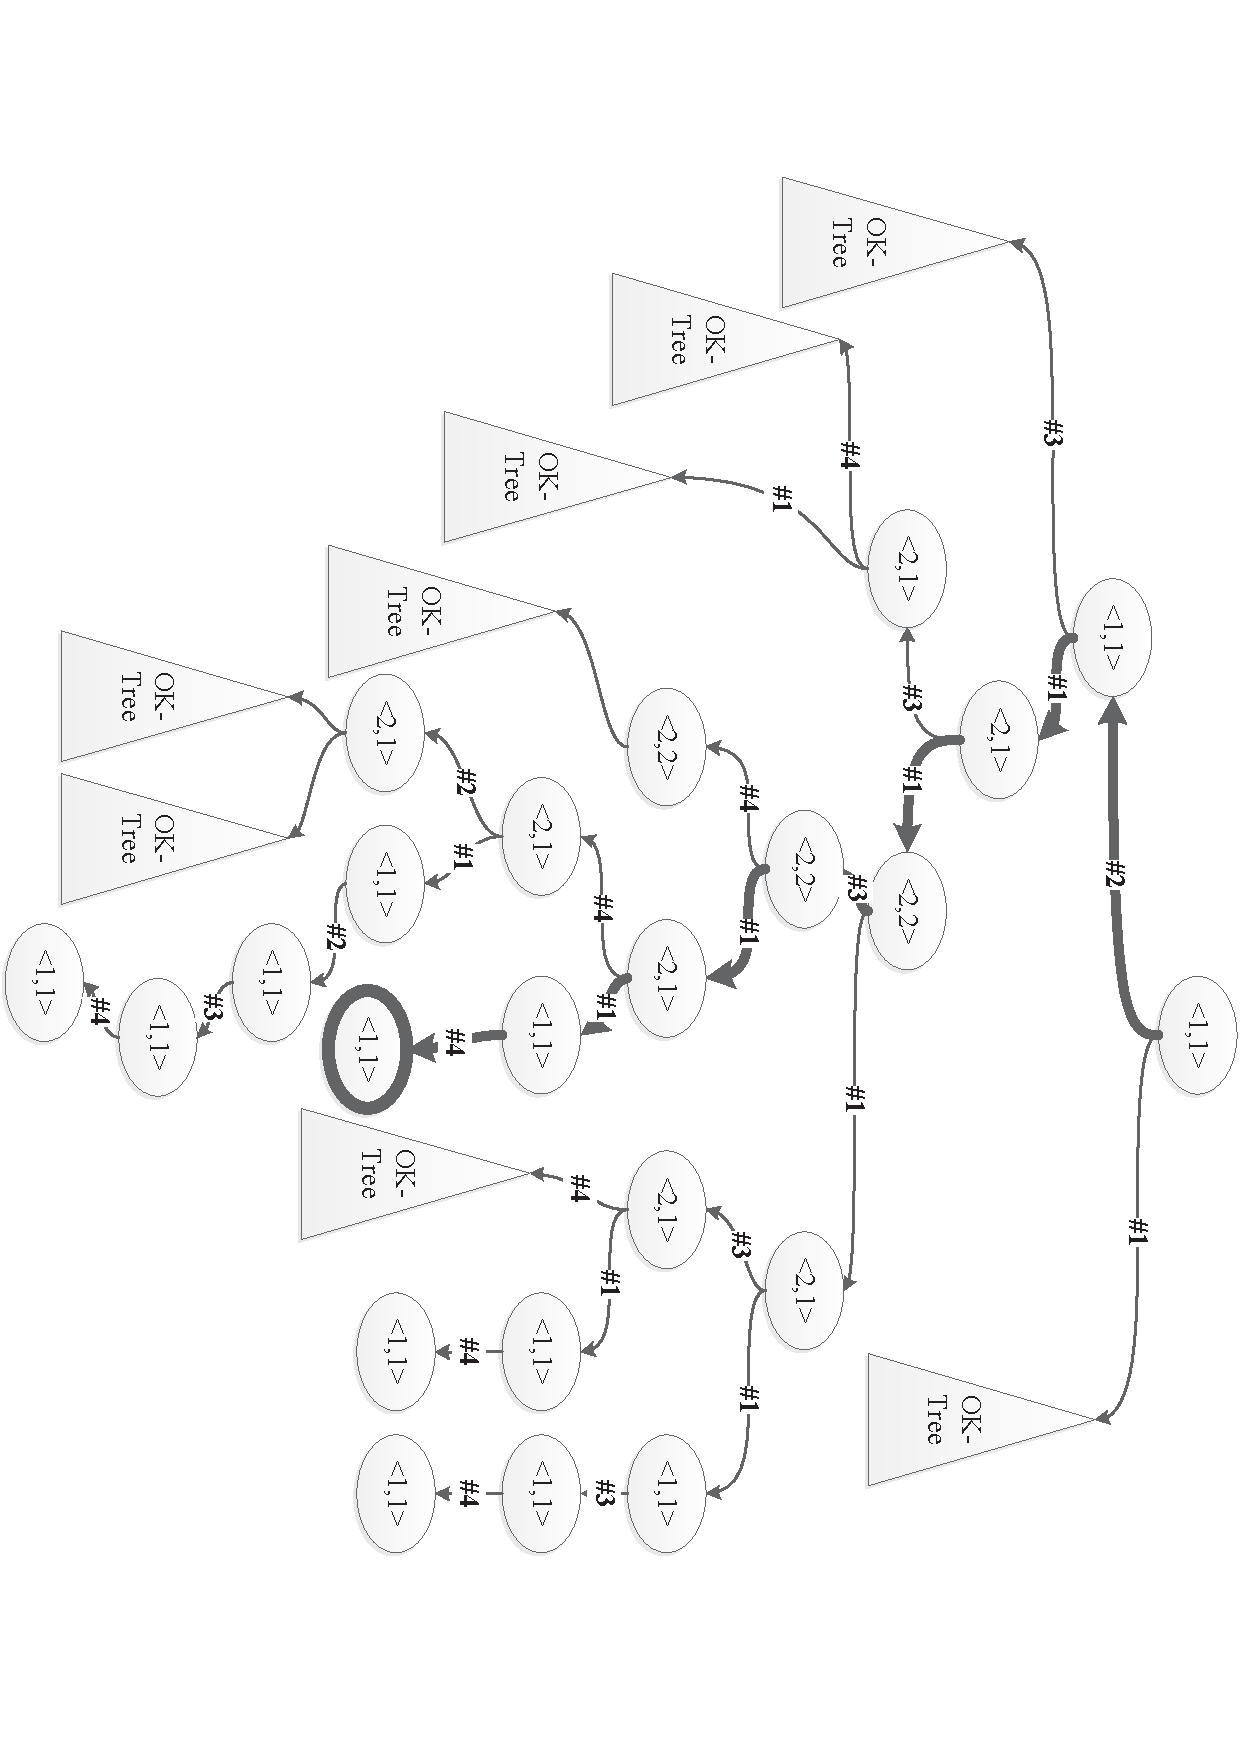
\includegraphics[height = 2.5in, width = 3in]{pssinttree.pdf}
\caption{Interleaving tree of PairSnapShot}\label{fig:interleavingtreeofpairsnapshot}
\end{wrapfigure}

In our system, a subtree $\mathcal{T}ree(N_{d})$ rooted at $N_d$ and holding a leaf set $N_{lf}$ can be grouped into one of the following categories:
\begin{itemize}
  \item \textit{OK}-tree --- all fine-grained traces are linearizable,\\
  $\forall l_f \left( l_f\in N_{lf} \rightarrow \mathcal{L}_n(l_f)\right)$
  \item \textit{ERR}-tree --- all fine-grained traces are non-linearizable,\\
  $\forall l_f \left(  l_f\in N_{lf} \rightarrow \neg \mathcal{L}_n(l_f)\right)$
  \item \textit{MIX}-tree --- both linearizable and non-linearizable fine-grained traces exist,\\
  $\exists l_{f1} ( l_{f1}\in N_{lf} \wedge \mathcal{L}_n(l_{f1})) \wedge  \exists l_{f2} (l_{f2}\in N_{lf} \wedge \neg \mathcal{L}_n(l_{f2}))$

\end{itemize}

\begin{myDef}[Node Labeling]\label{def:nodelabel}
Based on the categories of subtrees, a node $N_d$ can be labeled as one of the following symbols,
\begin{itemize}
  \item \textit{W}-node --- if $\mathcal{T}ree(N_d)$ is an \textit{OK}-tree.
  \item \textit{B}-node --- if $\mathcal{T}ree(N_d)$ is an \textit{ERR}-tree.
  \item \textit{G}-node --- if one subtree of $N_d$ is an \textit{OK}-tree, and the other is an \textit{ERR}-tree.
  \item \textit{GG}-node --- if two subtrees of $N_d$ are both \textit{MIX}-trees.
  \item \textit{WG}-node --- if one subtree of $N_d$ is an \textit{OK}-tree, and the other is a \textit{MIX}-tree.
  \item \textit{BG}-node --- if one subtree of $N_d$ is an \textit{ERR}-tree, and the other is a \textit{MIX}-tree.
\end{itemize}
\noindent where \textit{W} represents \textit{white}, \textit{B} represents \textit{black} and \textit{G} represents \textit{grey} actually. Fig. \ref{fig:labellabelnodes} illustrates this labeling rule.
\end{myDef}

\begin{figure}[!ht]
\centering
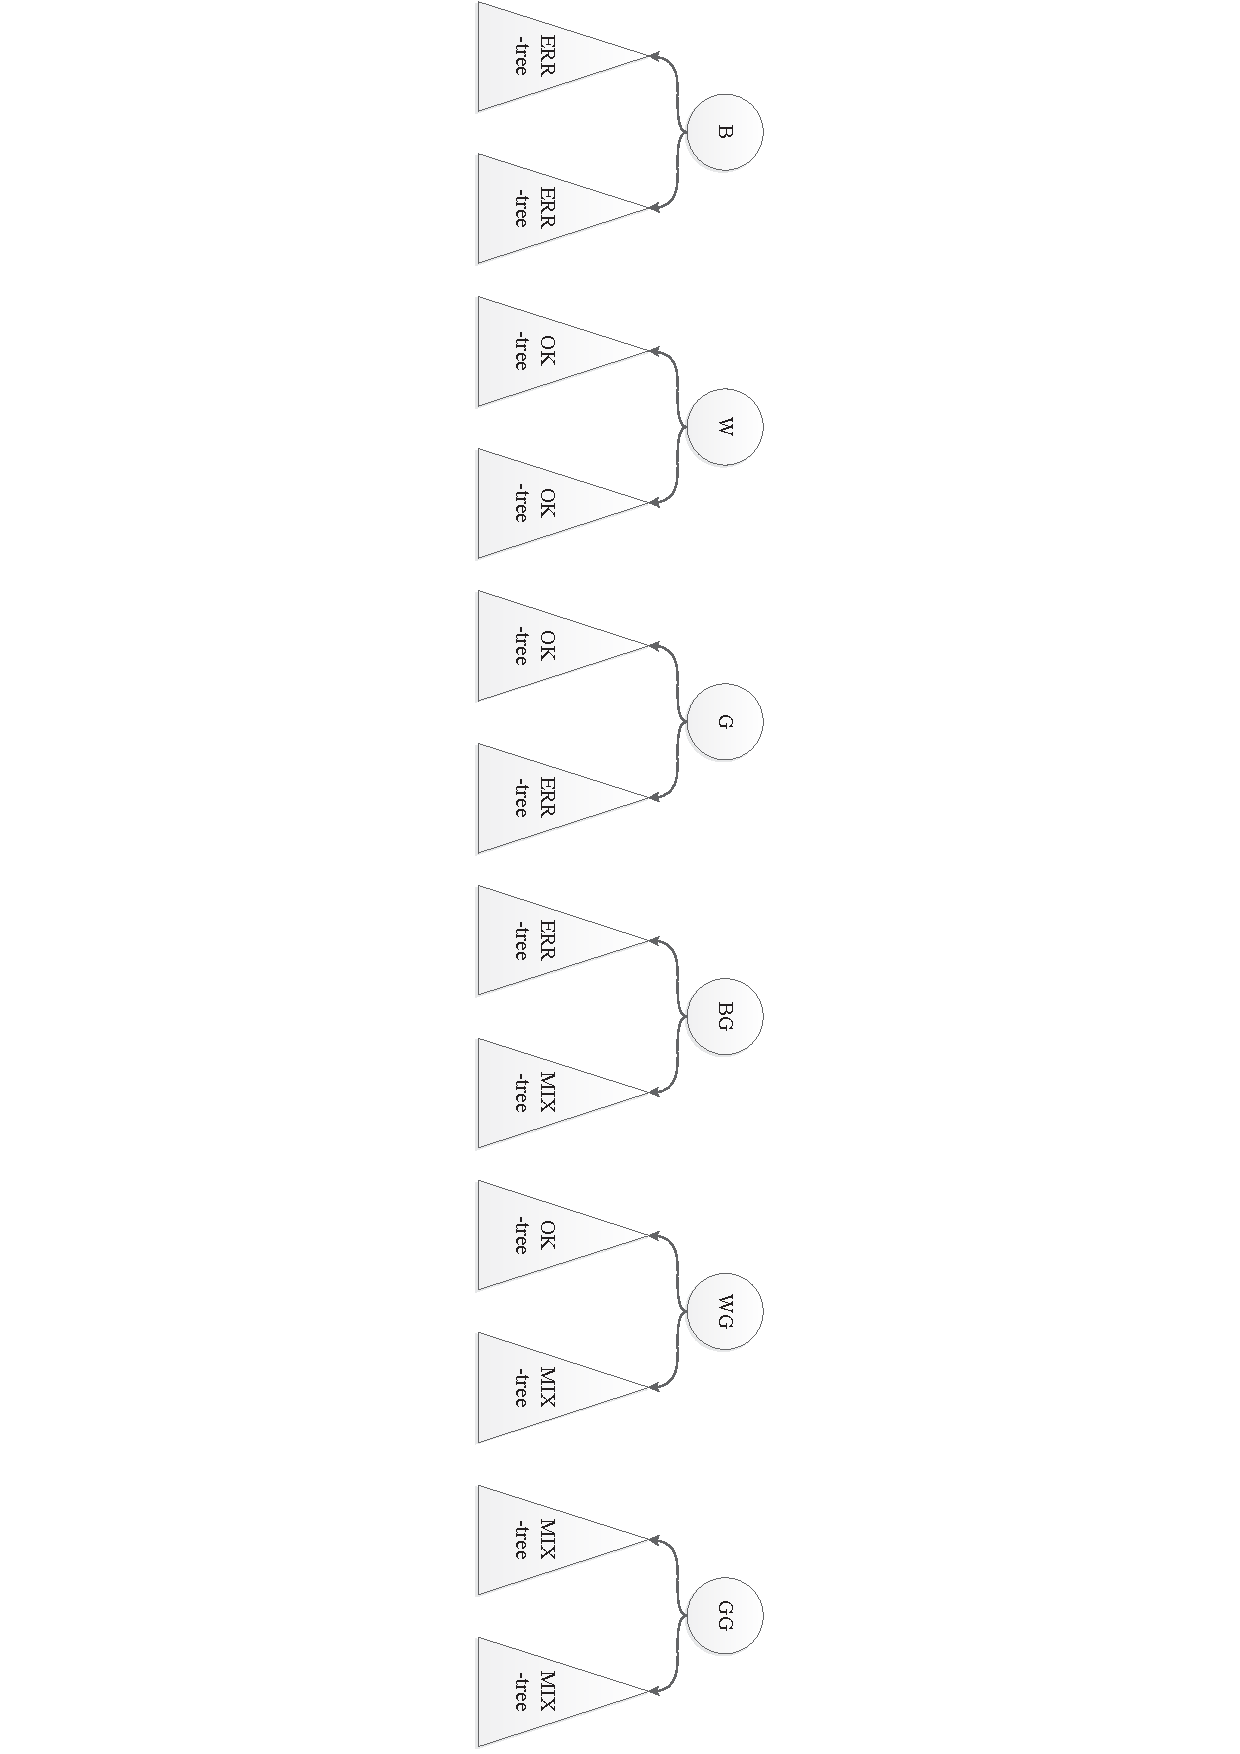
\includegraphics[width = 4.7in]{label.pdf}
\caption{Labels of nodes}\label{fig:labellabelnodes}
\end{figure}

The algorithm of labeling an interleaving tree is presented in Algorithm \ref{algo:labelinttree}. The function \textsc{LabelNode} recursively labels the nodes of a tree. Firstly, it checks whether the node being labeled has left or right child in line \{3,6,8,10\}, where $\mathtt{Left}(N_d)$ gets the left child of $N_d$, and $\mathtt{Right}(N_d)$ gets the right child. $!\mathtt{Left}(N_d)$ means that $N_d$ has no left child, and $!\mathtt{Right}(N_d)$ is in a similar way. So if both $!\mathtt{Left}(N_d)$ and $!\mathtt{Right}(N_d)$ are true, it means $N_d$ is a leaf and thus it is labeled depending on the linearizability of itself as line 3-5 shows. Otherwise, the node is labeled depending its left and right child as line 6-27 shows.



\begin{myTheo}[Completeness]
    Each node of the interleaving tree belongs to one kind of the nodes in Definition \ref{def:nodelabel}.
\end{myTheo}

%\begin{proof}
%    Since the interleaving tree in this section is a binary tree, each subtree $\mathcal{T}ree(N_d)$ has two subtrees. Each subtree belongs to one of the three kinds: \textit{OK}-tree, \textit{ERR}-tree and \textit{MIX}-tree. If we represents \textit{OK}-tree as \textit{O}, \textit{ERR}-tree as \textit{E} and \textit{MIX}-tree as \textit{M}, a node $N_d$ can be divided into 9 different kinds depending on the kinds of its left subtree and right subtree: \textit{OO}, \textit{EE}, \textit{OE}, \textit{EO}, \textit{MM}, \textit{OM}, \textit{MO}, \textit{EM}, \textit{ME}. Here, it is clear that \textit{OO} corresponds to \textit{W}-node, \textit{EE} corresponds to \textit{B}-node, \textit{OE} and \textit{EO} correspond to \textit{G}-node, \textit{MM} corresponds to \textit{GG}-node, \textit{OM} and \textit{MO} correspond to \textit{WG}-node, and \textit{EM} and \textit{ME} correspond to \textit{BG}-node.
%\end{proof}

\begin{algorithm}[ht]
\small
    \centering
    \caption{Labeling Interleaving Tree}\label{algo:labelinttree}
    \begin{algorithmic}[1]
        \State $\mathit{Label} = \set{W, B, G, GG, WG, BG}$
        \Function {LabelNode}{$N_d$}
            \If{$!\mathtt{Left}(N_d)  \& !\mathtt{Right}(N_d)$}
                \State \textbf{if} {$\mathcal{L}_n(N_d)$} \textbf{then} \Return $\mathit{W}$
                    %\State \Return $\mathit{W}$
                \State \textbf{else} \Return $\mathit{B}$
                    %\State \Return $\mathit{B}$
                %\State \textbf{end if}
            \ElsIf{$\mathtt{Left}(N_d)  \& !\mathtt{Right}(N_d)$}
                \State \Return \Call{LabelNode}{$\mathtt{Left}(N_d)$}
            \ElsIf{$!\mathtt{Left}(N_d)  \& \mathtt{Right}(N_d)$}
                \State \Return \Call{LabelNode}{$\mathtt{Right}(N_d)$}
            \Else
                \State $\mathit{Label_l} = $ \Call{LabelNode}{$\mathtt{Left}(N_d)$}
                \State $\mathit{Label_r} = $ \Call{LabelNode}{$\mathtt{Right}(N_d)$}
                \State \textbf{switch} {$\pair{\mathit{Label_l},\mathit{Label_r}}$}
                    \State \quad \textbf{case} {$\pair{\mathit{W,W}}$}:
                    \State \quad\quad\Return $\mathit{W}$
                        %\State \quad$\mathit{return}$ $\mathit{W}$
                   % \State \textbf{break}
                    \State \quad\textbf{case} {$\pair{\mathit{B,B}}$}:
                    \State \quad\quad\Return $\mathit{B}$
                       % \State \quad$\mathit{return}$ $\mathit{B}$
                    %\State \textbf{break}
                    \State \quad\textbf{case} {$\pair{\mathit{B,W}} | \pair{\mathit{W,B}}$}
                    \State \quad\quad\Return $\mathit{G}$
                       % \State \quad$\mathit{return}$ $\mathit{G}$
                  %  \State \textbf{break}
                    \State \quad\textbf{case} {$\pair{\mathit{(B|W|G)?G,W}} | \pair{\mathit{W,(B|W|G)?G}} $}: \State \quad\quad\Return $\mathit{WG}$
                        %\State \quad$\mathit{return}$ $\mathit{WG}$
                    %\State \textbf{break}
                    \State \quad\textbf{case} {$\pair{\mathit{(B|W|G)?G,B}} | \pair{\mathit{B,(B|W|G)?G}} $}: \State \quad\quad\Return $\mathit{BG}$
                        %\State \quad$\mathit{return}$ $\mathit{BG}$
                 %   \State \textbf{break}
                    \State \quad\textbf{case} {$\pair{\mathit{(B|W|G)?G,(B|W|G)?G}}$}:
                    \State \quad\quad\Return $\mathit{GG}$
                       % \State \quad$\mathit{return}$ $\mathit{GG}$
                  %  \State \textbf{break}
                \State \textbf{end switch}
            \EndIf
        \EndFunction
    \end{algorithmic}

\end{algorithm}

Actually, each node $N_d$ of an interleaving tree together with all of its out-edges corresponds to a data race $\mathsf{D} = \pair{\mathit{Var}, \se,\ce}$. The set $\mathit{Var}$ is a subset of the domain of $\mathit{State}$, where $\mathit{State}$ is represented by the value in a node $N_d$, $\se$ is a prefix composed of events represented by edges from the root to $N_d$, and $\ce$ contains all events $e$ each corresponding to an out-edge of $N_d$. Therefore, we can uniquely identify a data race by a node.

\begin{myTheo}[Identifying CDRS]\label{theo:idenfycdrs}
    A CDRS is equivalent to a subset of nodes in a root-to-leaf path, satisfying a regular expression form
    $$(W_g|B_g)^*(B_g|G)$$
    where $W_g,B_g,G$ respectively represent $\mathit{WG}$-node,$\mathit{BG}$-node,$\mathit{G}$-node.
\end{myTheo}





\begin{proof}



\begin{itemize}
\item Firstly we show that the node sequence following $(W_g|B_g)^*(B_g|G)$ in an interleaving tree is a CDRS.
From the definition of $W_g$-node, $B_g$-node, and $G$-node, it is obvious that the HLDRs composed by these 3 kinds of node and their out-edges all belong to the
data races described in the Definition~\ref{def:cdrs}.

\item Then we show that a CDRS appears as $(W_g|B_g)^*(B_g|G)$ in an interleaving tree.
According to Definition \ref{def:cdrs}, the two different cases for ``inverse'' consequences correspond to 
the $W_g$-node and $B_g$-node. Furthermore, since CDRS implies a linearizability fault $\mathcal{F}$, the ending of a CDRS 
should be that there exists an event whose win can lead all fine-grained trace non-linearizable, and that is just the case of $BG$-node 
and $G$-node, which corresponds to the expression in the theorem.
\end{itemize}
 
 \end{proof}








\begin{example}
Take a look at Fig.~\ref{fig:interleavingtreeofpairsnapshot}.  We label the tree according to Definition \ref{def:nodelabel}, resulting in a labeled tree presented in Fig. \ref{fig:labeledinterleavingtreepss}.  As we can see, the thickened path with a red leaf is non-linearizable, the nodes on which include a CDRS. The CDRS is shown by the sequence of yellow nodes, in the form of $\mathit{W_gW_gW_gW_gW_gG}$, which is accepted by the regular expression in Theorem \ref{theo:idenfycdrs}.

\end{example}


%Note that since the object considers its two memory locations (\texttt{d[0]} and \texttt{d[1]}) as a whole, $\mathit{Var}$ of each data race is composed of the two memory locations rather than one separately. That is reasonable, because an access to any memory location is actually an access to the array \texttt{d} as a whole, during which competitions between two threads exist.
\begin{wrapfigure}[18]{r}{0.6\textwidth}
\centering
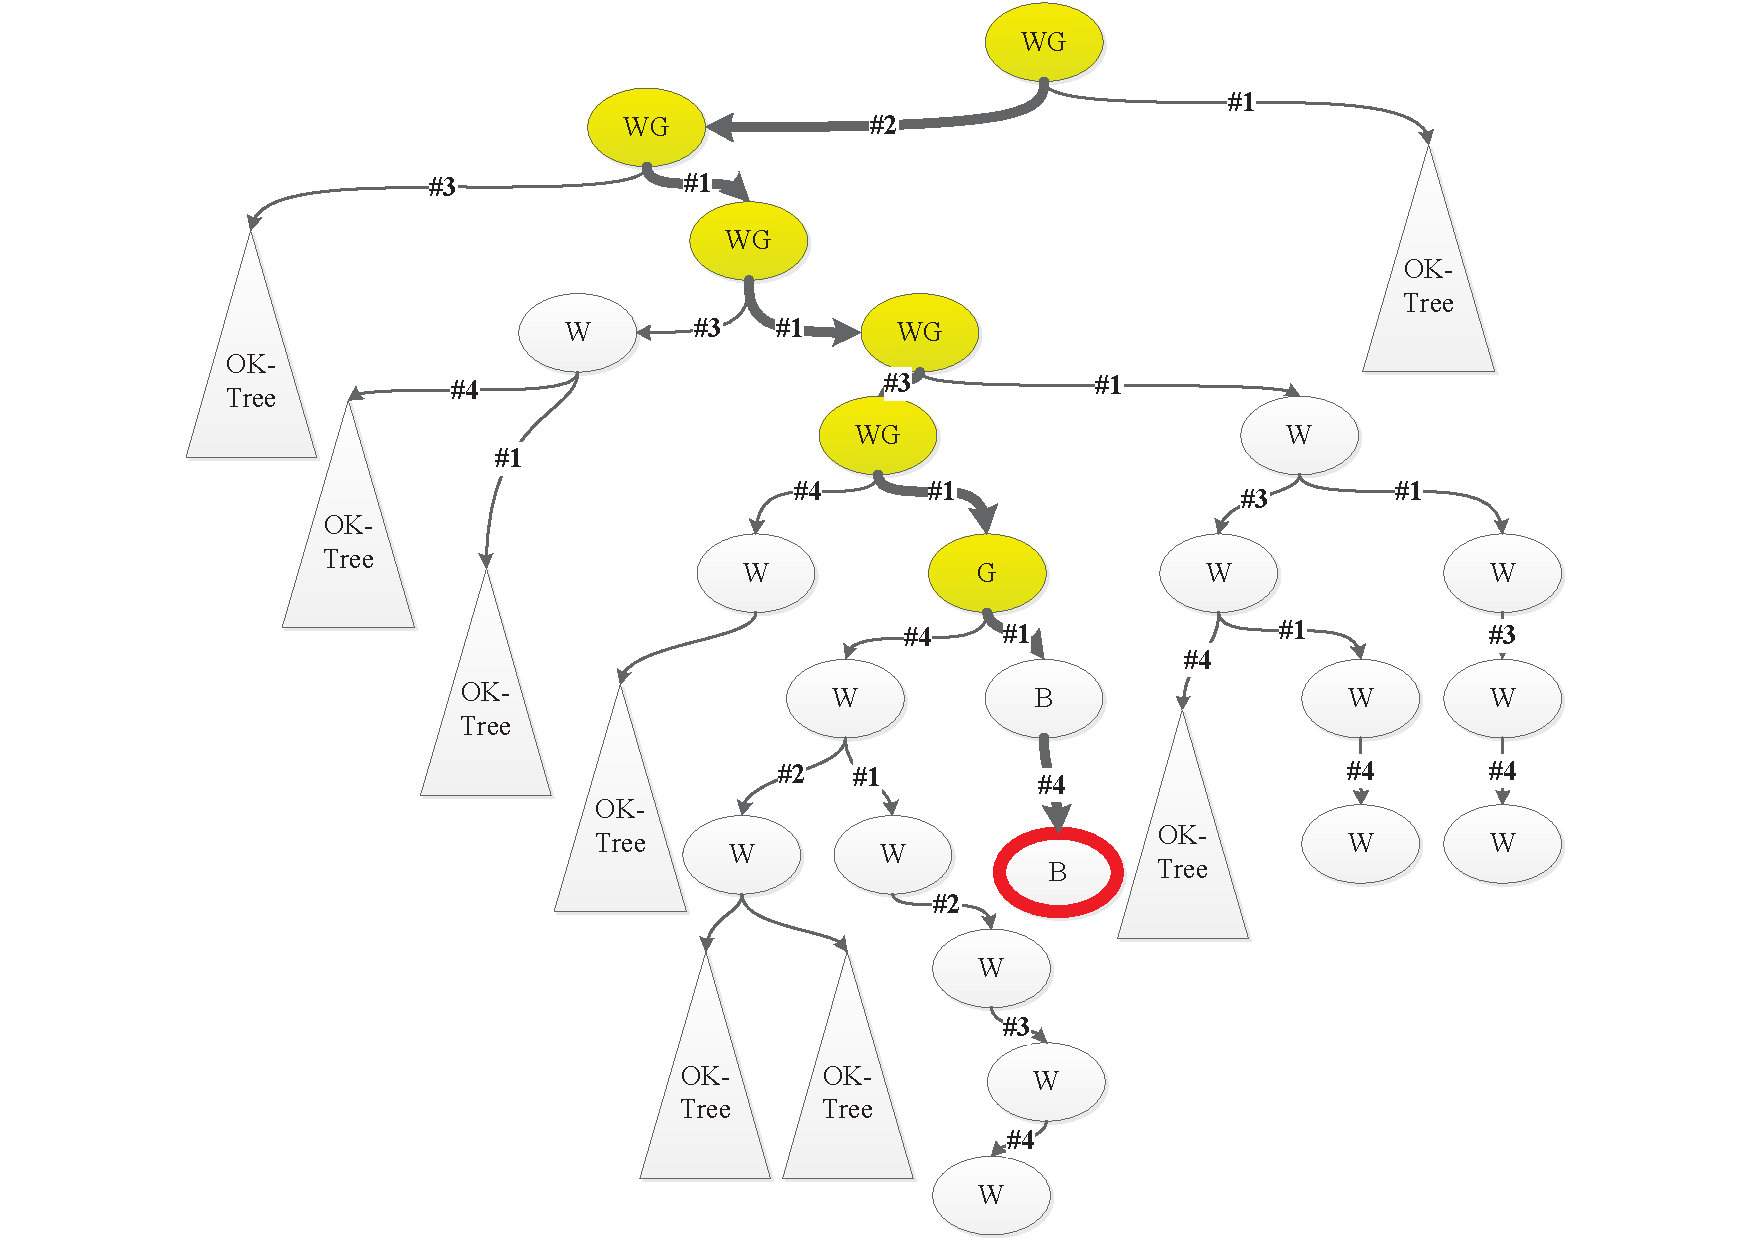
\includegraphics[height = 2.5in, width = 3in]{psslabeltree.pdf}
\caption{Labeled interleaving tree}\label{fig:labeledinterleavingtreepss}
\end{wrapfigure}









\section{Implementation and Evaluation}\label{sec:implementation}
We have integrated what we presented in Section \ref{sec:intertree} into a prototype tool called FGVT (Fine-grained VeriTrace), and experiments show that given a \textit{minimum test case} \cite{DBLP:conf/seke/ZhangWZ17}, our tool is able to localize the CDRS. In this section, we will give a brief introduction about our tool and experiments, and display the experiment results to show the power of FGVT.

\begin{table*}[t]
\centering
\caption{Evaluation Result}\label{tab:result}
\newcommand{\tabincell}[2]{\begin{tabular}{@{}#1@{}}#2\end{tabular}}
\begin{tabular}{lcccc}
\hline
Concur. object & Initial State & Operations & CDRS & Relating data race\\
%
\hline
LockFreeList &\{1\} &\tabincell{c}{thd1:$\mathtt{remove(1)}$\\thd2:$\mathtt{remove(1)}$} & $W_gG$ & \tabincell{c}{\texttt{curr.next.get()}\\ \texttt{attemptMark()}}\\
%
\hline
OptimisticQueue &\{1,2\} &\tabincell{c}{thd1:$\mathtt{poll()}$\\thd2:$\mathtt{poll()}$} & $G$ & \tabincell{c}{\texttt{head.getItem()}\\ \texttt{casHead()}}\\
% & \tabincell{c}{two \texttt{poll}s can return a same value\\ when every item in queue is different}
\hline
PairSnapshot &$\pair{1,1}$  &\tabincell{c}{thd1: $\mathtt{write(0,2),}$\\$\mathtt{write(1,2),}$\\$\mathtt{write(1,1),}$\\$\mathtt{write(0,1)}$\\thd2:$\mathtt{read()}$} & $W_g\{5\}G$ & \tabincell{c}{\texttt{d[i]=v}\\ \texttt{x=d[0],y=d[1]}\\ \texttt{if(x==d[0])}}\\
% & \tabincell{c}{\texttt{readPair} can return \\an inconsistent result}
\hline
Snark & \{1\}&\tabincell{c}{thd1:$\mathtt{popRight()}$\\thd2:$\mathtt{pushRight(2),}$\\ $\mathtt{popLeft()}$} & $W_gW_gG$ & \tabincell{c}{\texttt{rh=RightHat}\\ \texttt{DCAS(\&RightHat,...)}\\ \texttt{DCAS(\&LeftHat,...)}\\ \texttt{if(rh.R==rh)}}\\
\hline
SimpleList &\{1\} & \tabincell{c}{thd1:$\mathtt{add(3)}$\\thd2:$\mathtt{add(4)}$} & $B_g$ or $B_gG$ & \tabincell{c}{\texttt{pred.next=node}\\ \texttt{curr.val<v}}\\
\hline
LinkedList &\{1,5\}  &\tabincell{c}{thd1:$\mathtt{remove(1),}$\\ $\mathtt{add(9)}$\\thd2:$\mathtt{size()}$} & $W_gW_gG$ & \tabincell{c}{\texttt{node.next==tail}\\ \texttt{synchronized()}\{...\}}\\
\hline

\end{tabular}

\end{table*}

\subsection{Implementation}
Our tool FGVT is based on the framework of JavaPathFinder (JPF), which encapsulates a Java virtual machine and can be customized for use of model checking of Java programs. JPF is employed to generate interleaving trees, and it applies a dynamic reduction mechanism to eliminate duplicated program states and simplify the interleaving tree. Then, we label the tree based on Algorithm \ref{algo:labelinttree}, and report the CDRSes which cause linearizability faults. %Our tool is available on \textit{http://github.com/choshina/FGVT}.


%\subsection{Benchmark}\label{sec:benchmarks}
%In this section, we will introduce some concurrent objects in our experiment. 
%In addition to PairSnapShot, we also do experiments on many other concurrent objects, which have been proved to be non-linearizable by other tools.

%\begin{itemize}
 % \item LockFreeList \cite{herlihy2012art} --- It is a concurrent Set that violates linearizability when two $\mathtt{remove}$s compete to mark a bit without synchronization protection.
%  \item OptimisticQueue \cite{DBLP:conf/wdag/Ladan-MozesS04} --- It is a concurrent Queue that violates linearizability when two $\mathtt{poll}$ operations compete to get the head of the queue. Without proper synchronization between reading $\mathtt{head}$ pointer and modifying it, two $\mathtt{poll}$s may return the same value.

%  \item Snark \cite{DBLP:conf/spaa/DohertyDGFLMMSS04} --- It is a Deque with the use of DCAS (\textit{double-compare-and-swap}), and violates linearizability when the object has few elements and operations originally accessing different ends compete for the same memory location.

%  \item SimpleList \cite{DBLP:conf/pldi/VechevY08} --- It is a concurrent Set and the bug is typical. The $\mathtt{Add}$ function inserts a node by modifying the $\mathtt{next}$ pointer of its predecessor, but without protection, $\mathtt{next}$ may be modified by other threads leading the node removed from the list unexpectedly.
%  \item Operation $\mathtt{size}$ of Linked List --- As we know, $\mathtt{size}$ is used for counting the number of nodes in a list. However, if there is no synchronization, a situation that violates linearizability happens when $\mathtt{size}$ traverses the list, another thread preempts the execution and deletes a node which has been accessed and inserts a node at a position that has not been accessed, so $\mathtt{size}$ will return a value that is larger than the expected length.
%\end{itemize}



\subsection{Evaluation}
We evaluate our tool by 6 test cases either from prior work or from real applications.
The concurrent data structures and how the violations are caused have been introduced in last section. 
In our experiments, all the concurrent objects are executed by two threads, and the operations being tested with initial states of 
each concurrent object and arguments are listed in Columns 2-3 of Table \ref{tab:result}. 
%The CDRSes founded by our tool are presented in Column 4 of Table \ref{tab:result}.






%In Table \ref{tab:result}, Column 1 lists the concurrent objects introduced in Section \ref{sec:benchmarks}. Column 2 and 3 introduce the settings of our test cases, in which all test cases are small-scale but sufficient to trigger linearizability faults.

The node sequence patterns which are found based on the labeled interleaving tree is listed in Column 4 of Table \ref{tab:result}. 
As we present before, these patterns exactly correspond to the CDRSes of each test case, and here we got some conclusions from this experimental results:
\begin{itemize}
\item All the patterns follow the form of regular expression in Theorem \ref{theo:idenfycdrs}. 
\item Most of the test cases end with a $G$-node, and \textit{SimpleList} shows us a sequence ending with a $BG$-node.
\item We can see the case where not only one CDRS exists. 
\end{itemize}

Column 5 lists the relating source code corresponding to the CDRSes. The source code is acquired from the events participating in the CDRSes, and facilitates the bug repair a lot. For example, we can repair the linearizability faults in \textit{LockFreeList} by transforming \texttt{attemptMark} into \texttt{compareAndSet}, while there also exist other situations, such as \textit{PairSnapShot}, where we cannot point out exactly the modification of which instructions would lead the object linearizable, since all the data races participate in the CDRSes.

%Sometimes the source code is the position we should modify when we repair the linearizability faults such as \texttt{attemptMark} in \textit{LockFreeList}, but there also exist other situations, such as \textit{PairSnapShot}, where we cannot point out exactly the source code that leads the object to a non-linearizable state, since all data races participate in the CDRS.




%Scheduling is a key factor to decide the results in concurrent execution. In this paper, the scheduling information is implicated by the definition of fine-grained trace, since the events in a fine-grained trace contains the thread identifiers. \cite{burckhardt2010randomized,khoshnood2015concbugassist,Choi2000Deterministic} introduce some concurrent bug analysis techiniques based on scheduling.

\section{Conclusion}\label{sec:conclusion}
This paper proposes the notion of \textit{critical data race sequence} (\textit{CDRS}) that characterizes the root causes of linearizability faults based on a fine-grained trace model. A CDRS is a set of data races that are decisive to trigger linearizability faults. Therefore, the existence of a CDRS implies that a concurrent execution has potential to be non-linearizable. We also present a labeled interleaving tree model to support automated identification of CDRS. A tool called FGVT is then developed to automatically identify CDRSes and localize the causes of linearizability faults. Experiments have well demonstrated its effectiveness and efficiency.

This work reveals the pattern of the data races that are decisive on the linearizability of a trace. These data races can be mapped to certain parts of the source code. It would be interesting to establish a stronger relationship between CDRSes and the source code for the sake of bug analysis and repair.

\section{Acknowledgements}\label{sec:acknowledgement}

We thank the anonymous referees for their valuable comments. This work is partially supported by ERATO HASUO Metamathematics for Systems Design Project (No.~{JPMJER1603}), JST, the National Key Basic Research Program of China under the Grant No. 2014CB340701, the National Key Research and Development Program of China under the Grant No. 2017YFB0801900, and the CAS-INRIA Joint Research Program under the Grant No. GJHZ1844.

% ---- Bibliography ----
%
% BibTeX users should specify bibliography style 'splncs04'.
% References will then be sorted and formatted in the correct style.
%
 \bibliographystyle{splncs04}
 \bibliography{bare_conf}
%

\end{document}
